\documentclass[a4paper,11pt]{article}
\usepackage[margin=24mm]{geometry}
\usepackage{fontspec,amsmath,amssymb,amsthm,booktabs,graphicx}
\usepackage[hidelinks,unicode]{hyperref}
\usepackage{microtype}
\ifChinese
  \usepackage{xeCJK}
  \setCJKmainfont{NotoSerifCJKtc-Regular.otf}[Path=fonts/,
    BoldFont=NotoSerifCJKtc-Bold.otf,ItalicFont=NotoSerifCJKtc-Regular.otf,
    BoldItalicFont=NotoSerifCJKtc-Bold.otf]
  \setCJKmonofont{NotoSerifCJKtc-Regular.otf}[Path=fonts/,BoldFont=NotoSerifCJKtc-Bold.otf]
  \renewcommand{\abstractname}{摘要}
  \renewcommand{\proofname}{證明}
  \renewcommand{\refname}{參考文獻}
  \renewcommand{\figurename}{圖}
  \renewcommand{\tablename}{表}
  \newcommand{\bi}[2]{#2}
\else
  \newcommand{\bi}[2]{#1}
\fi
\newtheorem{thm}{\bi{Theorem}{定理}}
\newtheorem{lem}[thm]{\bi{Lemma}{引理}}
\newtheorem{cor}[thm]{\bi{Corollary}{推論}}
\theoremstyle{definition}
\newtheorem{prop}[thm]{\bi{Proposition}{命題}}
\newcommand{\abs}[1]{\left|#1\right|}
\newcommand{\Q}{\mathcal Q}
\newcommand{\ee}{\mathrm e}
\newcommand{\dd}{\,\mathrm d}
\setlength{\emergencystretch}{2em}
\raggedbottom
\newcommand{\papertitle}{\bi{Exact clusters and global transitions in periodic alternating Gaussian chains with a minimum spacing}{具最小間距的週期交替高斯鏈：精確聚簇與全域相變}}
\newcommand{\coordinator}{Research coordination: yuri77521}
\newcommand{\researchcredit}{AI research: OpenAI Codex (GPT-6.2 Astra)}
\newcommand{\projectcredit}{Independent Research Project}
\title{\papertitle}
\author{\textbf{\coordinator}\\\textbf{\researchcredit}\\\projectcredit}
\hypersetup{pdftitle={\papertitle},pdfauthor={\coordinator; \researchcredit; \projectcredit}}
\date{\bi{26 November 2026}{2026 年 11 月 26 日}}
\begin{document}
\maketitle
\begin{abstract}
\bi{We minimize the energy of a periodic chain with alternating unit charges and a Gaussian interaction, with a lower bound on each gap. For fixed even particle count and $\sum_{n\ge2}n^4q^{n^2-1}\le2/3$, an explicit small positive floor forces two exactly packed, balanced odd clusters with antipodal midpoints. We compute the minimum through fourth order. For six particles and every normalized width $7.99\le s\le9$, two simple decreasing curves partition the positive-floor parameter strip into centered, displaced and five-contact regimes, with a single uniform cell at the feasibility endpoint. The intervening phase widens on $[8,9]$. At the single parameter pair $(s,h)=(22,1/1000)$ the unique geometric shape instead has one triple and three single sites. The general contact theorem is analytic. The six-site global classifications combine analytic reductions with exhaustive rational interval certificates. Four algebraic declarations used in the small-gap analysis have Lean proofs.}{本文研究一條電荷正負交替、以高斯勢相互作用的週期鏈，並對每個間隙施加硬下限。對固定偶數粒子數及滿足 $\sum_{n\ge2}n^4q^{n^2-1}\le2/3$ 的寬度，當正下限小於一個明確界時，全部極小者恰由兩個緊密奇數簇組成，大小盡量均衡，中點對徑；最低能量可展開至四階。對六粒子及每個歸一化寬度 $7.99\le s\le9$，兩條嚴格下降的簡單根曲線把正下限參數帶分成對徑、偏移及五接觸三相，可行域終點僅有均勻構型；偏移相在 $[8,9]$ 上嚴格變寬。在單一參數點 $(s,h)=(22,1/1000)$，唯一幾何形狀變為一個緊三粒子簇及三個單粒子。一般粒子數的接觸鎖定有解析證明。六粒子全域分類結合解析歸約及窮盡的有理區間證書。小間距分析中的四個代數聲明另有 Lean 證明。}
\end{abstract}
\noindent\textbf{\bi{Keywords}{關鍵詞}}\quad
\bi{alternating charges, Gaussian energy, constrained crystallization, pitchfork bifurcation, interval arithmetic}{交替電荷、高斯能量、受約束結晶、叉形分岔、區間算術}
\section{\bi{Background and attribution}{背景與研究歸屬}}
\bi{A hard minimum spacing changes what a dense alternating chain can do. At zero spacing an adjacent positive and negative charge can cancel exactly. Once a positive floor is imposed, the residual interaction of the almost neutral pairs can select both the number of particles in each cluster and the positions of the individual particles. We ask for all minimizers at fixed period and particle count. Three different comparisons will matter: against a single trial cell, over the whole family of two packed triples, and over the entire feasible simplex.}{在稠密的交替鏈中，相鄰正負電荷可在零間距時完全抵消。給定正的硬下限後，近中性粒子對仍有相互作用，既可選出簇內的粒子數，也可固定個別粒子的位置。本文在固定週期及粒子數下求全部極小者。與單一試探構型比較、在整個緊雙三簇族取最小值，以及在全部可行間距單純形取最小值，是三個不同的命題。}

\bi{Bétermin, Knüpfer and Nolte introduced the alternating-chain energy and posed the equidistance conjecture for completely monotone profiles in the squared distance \cite{bkn}. The upstream manuscript gives a rigorous four-site Gaussian counterexample \cite{base}. A subsequent Lean proof compares the continuous four-site displacement family with the uniform cell for $0<q\le1/4$ \cite{prseven}. The dilute theorem \cite{dilute} proves equidistance for $\alpha(L/N)^2\ge4$. Its parameter is the squared dimensionless mean spacing. Here the period and particle count fix that mean while the independent floor can vary.}{Bétermin、Knüpfer 與 Nolte 定義交替鏈能量，並對距離平方的完全單調勢提出等距猜想 \cite{bkn}。上游論文已有嚴格的四粒子高斯反例 \cite{base}。其後的 Lean 證明在 $0<q\le1/4$ 比較了連續四粒子位移族與均勻構型 \cite{prseven}。稀薄區定理 \cite{dilute} 證明 $\alpha(L/N)^2\ge4$ 時的等距結晶，其參數為無因次平均間距的平方。本題的平均間距由週期及粒子數固定，硬下限則可獨立改變。}

\bi{At $q\le1/3$, the infimum manuscript \cite{infimum} established the collision dipole, semicircle stability, localization of each particle, the balanced odd split and the quadratic small-floor cost. Its trial state already had packed antipodal clusters. The four-site theorem recorded with Issue 5 \cite{four} proved exact packing at $s=4$, $0<h\le1/(8\pi)$ in our units. It used gap derivatives to obtain equality. Its larger-cell tests include centered triples and the five-contact trial. Circle rearrangement \cite{circle} and stability theory on compact groups \cite{riesz} provide the analytic background. Square-root displacement laws have precedents for bipartite trial lattices of a single species \cite{bipartite}.}{碰撞下確界論文 \cite{infimum} 已在 $q\le1/3$ 證明對徑偶極、半圓穩定性、逐粒子定位、均衡奇數分簇與小間距的二次能量代價，所採用的試探構型已是對徑緊雙簇。Issue 5 所附實驗室稿件的四粒子定理 \cite{four} 利用間距導數確定取等；換算本文單位，其範圍為 $s=4$、$0<h\le1/(8\pi)$。該研究的較大粒子數實驗包括居中三粒子簇與五接觸試探。圓周重排 \cite{circle} 和緊群穩定性理論 \cite{riesz} 提供解析背景；單一粒子種類的雙亞格子試探族已有平方根位移律的先例 \cite{bipartite}。}

\bi{The candidate contributions relative to these records are the quantified exact contact and antipodal locking for general even counts, the fourth-order coefficient, the global six-site phase strip including its two transition curves and widening interval, and a different global ground state at one outlying parameter pair. Attribution is relative to the fixed manuscripts and literature records preserved with the source index.}{相對於上述文獻，本項目可主張的候選增量為一般偶數粒子數的定量精確接觸與對徑鎖定、四次係數、六粒子的全域三相條帶及兩條相界與相寬，以及條帶外一點的另一種全域基態。原創性判斷限於研究索引凍結時本地保存的手稿與文獻記錄。}

\section{\bi{Model, normalization and equivalence}{模型、歸一化與等價關係}}
\bi{Fix $N=2m$, $L>0$ and $\alpha>0$. Write $x_j=X_j/L$, $x_{j+N}=x_j+1$, $\sigma_j=(-1)^j$, $g_j=x_{j+1}-x_j$. All $N$ gaps, including the last, satisfy $g_j\ge h=h_{\rm phys}/L$, $\sum g_j=1$. The mean gap is $1/N$. We use}{固定 $N=2m$、$L>0$ 及 $\alpha>0$。令 $x_j=X_j/L$、$x_{j+N}=x_j+1$、$\sigma_j=(-1)^j$、$g_j=x_{j+1}-x_j$。包括跨週期間隙在內，全部 $N$ 個間隙均滿足 $g_j\ge h=h_{\rm phys}/L$、$\sum g_j=1$。平均間距為 $1/N$。記}
\begin{equation}\label{eq:model}
 s=\alpha L^2,\quad q=\ee^{-\pi^2/s},\quad c=\sqrt{\pi/s},\quad
 \theta_j=2\pi x_j,\quad \eta=2\pi h,\quad
 G_s(d)=\sum_{p\in\mathbb Z}\ee^{-s(d+p)^2}.
\end{equation}
\bi{The ordered energy per particle, and its Fourier representation by Poisson summation, are}{對每粒子計的有向能量及由 Poisson 求和得到的 Fourier 表示為}
\begin{equation}\label{eq:energy}
 E_s=1-\frac1N\sum_{i,j}\sigma_i\sigma_j G_s(x_j-x_i)
 =1-\frac{2c}{N}\sum_{n\ge1}q^{n^2}|P_n|^2,\qquad
 P_n=\sum_j\sigma_j\ee^{in\theta_j}.
\end{equation}
\bi{Neutrality removes the constant Fourier mode. The leading 1 removes exactly the central self interaction per particle. Images with the same label in other cells remain. Total energy is $NE_s$. The unordered-pair score $W=\sum_{i<j}\sigma_i\sigma_j G_s(x_j-x_i)$ satisfies $E_s=1-G_s(0)-2W/N$. Derivative series converge absolutely and uniformly on compact parameter sets with $s>0$. For $0<h\le1/N$, the simplex modulo translation is compact. We write $M_N(h;s)$ for its attained minimum. At $h=0$, distinguish the open strictly ordered class from the compact collision closure. Rotations translate all sites. Even cyclic relabelings preserve species; an odd shift with the first sign reset reverses all charges. Reflections can preserve species; global sign reversal is a separate equivalence.}{電中性消去 Fourier 零模。常數 1 恰刪去每粒子的中央自身相互作用，其餘週期的同標號像仍計入。總能量為 $NE_s$；若 $W=\sum_{i<j}\sigma_i\sigma_j G_s(x_j-x_i)$ 對無序粒子對求和，則 $E_s=1-G_s(0)-2W/N$。各階導數級數於 $s>0$ 的緊參數集上絕對一致收斂。當 $0<h\le1/N$，模平移的可行單純形為緊集，最低值記作 $M_N(h;s)$。在 $h=0$ 時分別考慮嚴格有序類和容許碰撞的閉包。旋轉即全體平移。偶數步循環重標保留種類；奇數步重標並重置首電荷相當於整體換號。可另取保號反射，並明確區分是否容許整體換號。}


\section{\bi{From collision stability to exact contacts}{由碰撞穩定性到精確接觸}}
\begin{thm}\label{th:lock}
\bi{Let $N=2m\ge4$, $C=1+3\pi m^2$, $R=\sum_{n\ge2} n^4q^{n^2-1}\le2/3$. If $0<\eta\le1/(NC^2)$, all minimizers consist of two packed progressions of steps $h$, antipodal midpoints and counts $2k+1,2l+1$, where $k+l=m-1$, $|k-l|\le1$. Each outer gap is $1/2-(m-1)h$. There is one species-preserving isometry orbit for $k=l$, two for $k\ne l$, exchanged by global sign reversal. The width condition holds for $q\le17/50$. For $N=2$ under the same width condition the antipodal pair minimizes uniquely up to rotation for every feasible floor.}{設 $N=2m\ge4$、$C=1+3\pi m^2$、$R=\sum_{n\ge2}n^4q^{n^2-1}\le2/3$。若 $0<\eta\le1/(NC^2)$，全部極小者由兩列公差恰為 $h$ 的緊簇組成，中點對徑，粒子數分別為 $2k+1,2l+1$，其中 $k+l=m-1$、$|k-l|\le1$。兩個外間隙均為 $1/2-(m-1)h$。在保號等距變換下，$k=l$ 時有一個軌道，$k\ne l$ 時有兩個，整體換號互換二者。$q\le17/50$ 足以滿足寬度條件。對 $N=2$，在相同寬度條件下，任一可行下限均由對徑對唯一取等，模整體平移。}
\end{thm}
\begin{proof}
\bi{Write $a_n=q^{n^2-1}$ and $K(u)=\sum_{n\ge1}a_n\cos(nu)$. The ratio bound $R\le16q^3/(1-(3/2)^4q^5)<2/3$ holds at and below $17/50$. Under the stated $R$ hypothesis, $\|K''\|_\infty,\|K^{(4)}\|_\infty<2$, $K''(\pi)\ge1-R/4\ge5/6$, and $D=K''(\pi)-K''(0)=2\sum_{n\ {\rm odd}}n^2a_n$ obeys $2\le D<4$. All sums over parity below use positive frequencies.}{置 $a_n=q^{n^2-1}$、$K(u)=\sum_{n\ge1}a_n\cos(nu)$。相鄰項比值給出 $R\le16q^3/(1-(3/2)^4q^5)<2/3$，適用於 $q\le17/50$。在定理的 $R$ 條件下，$\|K''\|_\infty,\|K^{(4)}\|_\infty<2$、$K''(\pi)\ge1-R/4\ge5/6$、$D=K''(\pi)-K''(0)=2\sum_{n\ {\rm odd}}n^2a_n$ 滿足 $2\le D<4$。奇偶頻率和均只取正整數。}

\bi{\emph{Localization.} Let $A$ consist of the arcs from a positive site to the next negative site, so $\mu=(\mathbf1_A)'=\sum\sigma_j\delta_{\theta_j}$. Integration by parts twice gives $Q_v(A)=\iint v(u-w)\dd\mu(u)\dd\mu(w)=\int_{A^2}-v''(u-w)\dd u\dd w$. For $v=K-\cos/3$, both $v$ and $-v''$ decrease weakly on $[0,\pi]$: the first-mode derivative dominates the tails by $|\sin(nu)|\le n\sin u$. Add a constant to $-v''$ to make it positive. Circle rearrangement \cite[Thm.~4.1]{circle} bounds the integral by that on an arc of equal length $b$; the constant cancels. Its value is $2[v(0)-v(b)]$, maximal at $b=\pi$. The reserved kernel contributes $|z|^2/3$, $z=\int_A e^{iu}\dd u$. With $H$ a semicircle and $I_N=1-2[G_s(0)-G_s(1/2)]/N$, this yields}{\emph{定位。} 令 $A$ 為從正粒子至下一負粒子的有向弧之聯集，則 $\mu=(\mathbf1_A)'=\sum\sigma_j\delta_{\theta_j}$。兩次分部積分得 $Q_v(A)=\iint v(u-w)\dd\mu(u)\dd\mu(w)=\int_{A^2}-v''(u-w)\dd u\dd w$。取 $v=K-\cos/3$，由 $|\sin(nu)|\le n\sin u$ 及尾項界，$v$ 和 $-v''$ 在 $[0,\pi]$ 上皆非增。為 $-v''$ 加常數使其為正，圓周重排 \cite[定理 4.1]{circle} 給出同長度 $b$ 的單弧上界，並可抵消所加常數。單弧的值 $2[v(0)-v(b)]$ 在 $b=\pi$ 最大。保留的一階核貢獻 $|z|^2/3$，其中 $z=\int_A e^{iu}\dd u$。記半圓為 $H$，$I_N=1-2[G_s(0)-G_s(1/2)]/N$，則}
\begin{equation}\label{eq:deficit}
 F=\frac{N(E_s-I_N)}{2cq}=Q_K(H)-Q_K(A)\ge (4-|z|^2)/3 .
\end{equation}
\bi{Choose $H$ where $\cos(u-\arg z)>0$ (any phase for $z=0$). Then $J=\int_{A\triangle H}|\cos(u-\arg z)|\dd u=2-|z|\le3F/2$. Placing measure $b$ nearest the two zeros gives $J\ge4[1-\cos(b/4)]$ for $b=|A\triangle H|$. Thus at zero floor equality requires and suffices that the signed jumps reduce to an antipodal dipole. Splitting an odd cluster about one end gives strictly ordered approximants, so this is the open-class infimum. For $N>2$ equality needs collisions, whereas the two-site dipole is feasible at all floors.}{取 $\cos(u-\arg z)>0$ 所在的半圓 $H$（$z=0$ 時相位任取）。則 $J=\int_{A\triangle H}|\cos(u-\arg z)|\dd u=2-|z|\le3F/2$。把長度 $b$ 集中在兩零點附近可得 $J\ge4[1-\cos(b/4)]$，其中 $b=|A\triangle H|$。故在零下限的閉包中，帶號跳躍抵消後恰為對徑偶極是取等的充要條件。將一端的奇數簇拆開即有嚴格有序的逼近列，所以 $I_N$ 也是開類下確界。$N>2$ 時取等須有碰撞，兩粒子對徑構型則在每個可行下限取等。}

\bi{For a packed odd block put $B_j(w)=\sum_{p=-j}^j(-1)^{j+p}\cos(pw)$. Pairing consecutive cosines gives $|1-B_j(w)|\le j(j+1)w^2/2$, since $2|\cos((r-1)w)-\cos(rw)|\le(2r-1)w^2$. The antipodal balanced trial has squared amplitude $[B_k(n\eta)-(-1)^n B_l(n\eta)]^2$. Even modes cannot increase its deficit and $4-y^2\le4(2-y)$ for odd-mode amplitude $y=B_k+B_l$. Hence $F_{\rm trial}\le D A_m\eta^2$, $A_m=k(k+1)+l(l+1)=\lfloor m^2/2\rfloor$. Any minimizer satisfies $J\le3m^2\eta^2$. Rotate $H$ to $(0,\pi)$. If a jump lies distance $r\ge\eta$ from the nearer end, one of the two adjacent intervals of length $\eta/2$ belongs to the discrepancy. Since $\sin u\ge2u/\pi$ for $0\le u\le\pi/2$, $J\ge(\eta/\pi)(r-\eta/2)$. Every site thus lies within $C\eta$ of an endpoint. Outside the two neighborhoods the indicators agree: otherwise an intervening middle quarter-circle contributes $\sqrt2>3m^2\eta^2$. Here $C\eta<\pi/4$. The net jumps in the two neighborhoods are $+1,-1$, so both blocks are odd.}{令緊奇數簇的振幅 $B_j(w)=\sum_{p=-j}^j(-1)^{j+p}\cos(pw)$。相鄰餘弦配對，利用 $2|\cos((r-1)w)-\cos(rw)|\le(2r-1)w^2$，得 $|1-B_j(w)|\le j(j+1)w^2/2$。均衡對徑試探的振幅平方為 $[B_k(n\eta)-(-1)^n B_l(n\eta)]^2$。偶模不會增加虧損，奇模取 $y=B_k+B_l$ 有 $4-y^2\le4(2-y)$。故 $F_{\rm trial}\le D A_m\eta^2$，$A_m=k(k+1)+l(l+1)=\lfloor m^2/2\rfloor$。每個極小者有 $J\le3m^2\eta^2$。將 $H$ 旋至 $(0,\pi)$。若跳點距較近端點 $r\ge\eta$，則其左右長 $\eta/2$ 的兩段中有一段全屬差異集；在 $[0,\pi/2]$ 用 $\sin u\ge2u/\pi$ 得 $J\ge(\eta/\pi)(r-\eta/2)$。故各粒子距端點至多 $C\eta$。兩鄰域外指示函數一致，否則中間四分之一圓貢獻 $\sqrt2>3m^2\eta^2$；此處 $C\eta<\pi/4$。兩端鄰域的淨跳躍是 $+1,-1$，各簇均為奇數。}

\bi{\emph{Selection and contact.} In each cluster use offsets $u_i$ from its assigned antipode and normalize the initial sign to $+1$. Set $P=\sum(-1)^iu_i$, $V=\sum(-1)^iu_i^2-P^2$. Write the gaps $a_1,b_1,\ldots,a_j,b_j$. Consecutive differences of squares and cancellation of $P^2$ give}{\emph{分簇與接觸。} 以各自的對徑端點為原點，記偏移 $u_i$，將各簇的起始符號歸一為正。置 $P=\sum(-1)^iu_i$、$V=\sum(-1)^iu_i^2-P^2$，簇內間隙依次為 $a_1,b_1,\ldots,a_j,b_j$。相鄰平方作差並減去 $P^2$ 得}
\begin{equation}\label{eq:mom}
 P=u_0+\sum_r b_r,\qquad V=2\sum_{r=1}^j b_r\sum_{i=1}^r a_i\ge j(j+1)\eta^2 .
\end{equation}
\bi{Each gap derivative of $V$ is at least $2\eta$. In the Taylor expansion of each ordered pair at $0$ or $\pi$, odd derivatives vanish and the offset is at most $2C\eta$. The signed sum of squared differences within a cluster is $2V$; across the two clusters with initial signs normalized it is $V_0+V_\pi+(P_0-P_\pi)^2$. Counting both cross directions gives}{每個間隙的 $V$ 偏導數皆至少為 $2\eta$。在 $0$ 或 $\pi$ 處對各有向粒子對作 Taylor 展開，奇階導數為零，偏移不逾 $2C\eta$。同簇的帶號差平方和為 $2V$，異簇起始符號各自歸一後為 $V_0+V_\pi+(P_0-P_\pi)^2$。將異簇兩個方向計入，得}
\begin{equation}\label{eq:taylor}
 F=D(V_0+V_\pi)+K''(\pi)(P_0-P_\pi)^2+\mathcal R,\qquad
 |\mathcal R|\le\tfrac43 N^2C^4\eta^4 .
\end{equation}
\bi{An unbalanced pair increases the sum of the two $j(j+1)$ by at least two. The error is at most $4\eta^2/3<2D\eta^2$, contradicting the trial bound. To vary gap $p$ at fixed signed first moments, use velocity $\mathbf1_{i\ge p}-\mathbf1_{p\ {\rm even}}$ in that cluster, zero outside. A small decrease of a slack gap draws its suffix or prefix inward, preserving the other internal gaps and widening one outer gap. All relative velocities have modulus at most one. Expanding $K'$ with remainder $\|K^{(4)}\|_\infty(2C\eta)^3/6$ per pair gives $\partial_p F\ge2D\eta-(8/3)N^2 C^3\eta^3>0$. A slack gap contradicts minimality.}{若兩簇不均衡，兩項 $j(j+1)$ 的和至少增加二。餘項至多 $4\eta^2/3<2D\eta^2$，與試探上界矛盾。改變第 $p$ 個間隙但固定兩簇帶號一階矩，取本簇粒子速度 $\mathbf1_{i\ge p}-\mathbf1_{p\ {\rm even}}$，其餘為零。將鬆弛間隙稍微縮短只令其前綴或後綴內移，保持其他內間隙並增大一個外間隙。相對速度絕對值至多為一；直接展開 $K'$，逐對餘項至多 $\|K^{(4)}\|_\infty(2C\eta)^3/6$，故 $\partial_p F\ge2D\eta-(8/3)N^2 C^3\eta^3>0$。鬆弛間隙與極小性矛盾。}

\bi{\emph{Midpoints.} In a packed odd block $P$ equals its midpoint offset. At separation $\pi+v$ the variable part of $F$ is twice the alternating cross sum of $K(\pi+v+(j-i)\eta)$, even in $v$ by reflection. On the segment to zero every argument stays within $2C\eta$ of $\pi$ by convexity, and both outer gaps stay feasible. The signed coefficients have sum one before doubling. Bounding the change in each $K''$ by $\|K^{(4)}\|_\infty(2C\eta)^2/2$ and the number of terms by $N^2/4$ gives $F_{vv}\ge2K''(\pi)-2/C^2>0$. Hence $v=0$. Equal counts allow a half turn to interchange signs; unequal counts distinguish the size carrying positive net charge, even under reflection. Existence and sign symmetry realize both assignments.}{\emph{中點。} 在緊奇數簇中 $P$ 等於中點偏移。當中點相隔 $\pi+v$，$F$ 的可變部分為 $K(\pi+v+(j-i)\eta)$ 之交替跨簇和的兩倍。反射使其為 $v$ 的偶函數。沿 $v$ 到零的線段，各核自變量距 $\pi$ 不逾 $2C\eta$，兩個外間隙保持可行，兩者均由端點及凸性得到。倍乘前各係數的帶號和為一。每項 $K''$ 的變化至多 $\|K^{(4)}\|_\infty(2C\eta)^2/2$，項數不逾 $N^2/4$，故 $F_{vv}\ge2K''(\pi)-2/C^2>0$，必有 $v=0$。兩簇同大時平移半圈互換電荷；不同大時，帶正淨電荷的簇大小在保號反射下仍可區分。極小者的存在性與換號對稱性保證兩種指派皆取等。}
\end{proof}

\begin{cor}\label{th:energy}
\bi{Under Theorem~\ref{th:lock}, put $A=k(k+1)$, $B=l(l+1)$ and $S_{p,o},S_{p,e}=\sum n^p q^{n^2}$ over odd and even $n$, respectively. Then}{在定理~\ref{th:lock} 的條件下，記 $A=k(k+1)$、$B=l(l+1)$，並以 $S_{p,o},S_{p,e}$ 分別表示 $\sum n^p q^{n^2}$ 的奇、偶頻率和。則}
\begin{align}
 M_N &=1-\frac{2c}{N}\sum_{n\ge1}q^{n^2}[B_k(n\eta)-(-1)^nB_l(n\eta)]^2,\label{eq:exact}\\
 M_N &= I_N+\frac{4c(A+B)}N S_{2,o}\eta^2 \notag\\
 &\quad-\frac{2c}{N}\left[\left(\frac{(A+B)^2}{4}+
 \frac{A(A-1)+B(B-1)}6\right)S_{4,o}+\frac{(A-B)^2}4 S_{4,e}\right]\eta^4+O(\eta^6).\label{eq:fourth}
\end{align}
\end{cor}
\begin{proof}
\bi{Insert the minimizing coordinates in \eqref{eq:energy}. Pairing the outer terms in the finite exponential sum gives $B_j(u)=2\cos(ju)-B_{j-1}(u)$, $B_0=1$. Induction gives $B_k(u)=1-Au^2/2+A(A-1)u^4/24+O(u^6)$. Squaring the sum and difference yields \eqref{eq:fourth}. The trigonometric polynomials have bounded sixth derivatives, and the sixth Gaussian moment is finite at fixed $s,N$. For six sites $A=B=2$, hence the quadratic and quartic coefficients are $(8c/3)S_{2,o}$ and $-(14c/9)S_{4,o}$.}{將極小構型代入式 \eqref{eq:energy}。取有限指數和的兩端得遞推 $B_j(u)=2\cos(ju)-B_{j-1}(u)$、$B_0=1$。歸納得 $B_k(u)=1-Au^2/2+A(A-1)u^4/24+O(u^6)$，分別對和、差平方即得式 \eqref{eq:fourth}。三角多項式的六階導數有界，固定 $s,N$ 時高斯六階矩有限。六粒子有 $A=B=2$，二次、四次係數分別為 $(8c/3)S_{2,o}$ 與 $-(14c/9)S_{4,o}$。}
\end{proof}


\section{\bi{Motion of two packed triples}{緊雙三簇的相對位移}}
\bi{For six sites put $b=1/2-3h$ and introduce the entire closed family}{對六粒子令 $b=1/2-3h$，考慮整個閉構型族}
\begin{equation}\label{eq:y}
 Y(h,t)=(0,h,2h,\tfrac12+t,\tfrac12+t+h,\tfrac12+t+2h),\qquad |t|\le b .
\end{equation}
\bi{The other two gaps are $1/2-2h\pm t$. Write $x=\cos\eta$, $y=1-\cos(2\pi t)$, $y_b=1-\cos(2\pi b)$, $A_n=2T_n(x)-1$; $T_n(\cos v)=\cos(nv)$ and $T_n'=nU_{n-1}$. Subtracting the centered energy in \eqref{eq:energy} gives}{另兩間隙為 $1/2-2h\pm t$。令 $x=\cos\eta$、$y=1-\cos(2\pi t)$、$y_b=1-\cos(2\pi b)$、$A_n=2T_n(x)-1$，此處 $T_n(\cos v)=\cos(nv)$、$T_n'=nU_{n-1}$。利用式 \eqref{eq:energy} 減去對徑能量得}
\begin{align}
 E_s(Y(h,t))-E_s(Y(h,0))&=(4cq/6)\Phi(y),\notag\\
 \Phi(y)&=\sum_{n\ge1}(-1)^na_n A_n^2[T_n(1-y)-1],\qquad a_n=q^{n^2-1}.\label{eq:phi}
\end{align}
\begin{thm}\label{th:face}
\bi{For every $0<q\le17/50$ the entire family \eqref{eq:y} has the minimizers in Table~\ref{tab:phases}. Both thresholds are simple, real analytic and strictly decreasing in $s$; $1/8<h_c<h_b<1/6$.}{對每個 $0<q\le17/50$，整個構型族 \eqref{eq:y} 的極小者見表~\ref{tab:phases}。兩條臨界曲線皆為簡單根，對 $s$ 實解析且嚴格遞減，並有 $1/8<h_c<h_b<1/6$。}
\end{thm}
\par
\begin{table}[tbp]\centering
\caption{\bi{Minimizing displacements on the packed face. Theorem~\ref{th:strip} establishes globality on the stated strip.}{緊雙簇面上的全部極小位移；定理~\ref{th:strip} 證明其在指定條帶的全域性。}}\label{tab:phases}
\begin{tabular}{lll}\toprule
\bi{Floor}{下限} & \bi{Displacement}{位移} & \bi{Contact pattern}{接觸形態}\\\midrule
$0<h\le h_c$ & $0$ & \bi{two antipodal triples}{兩個對徑緊三簇}\\
$h_c<h<h_b$ & $\pm t_*,\quad 0<t_*<b$ & \bi{two unequal slack gaps}{兩個不等的鬆弛外間隙}\\
$h_b\le h<1/6$ & $\pm b$ & \bi{five consecutive contacts}{五個連續接觸}\\
$h=1/6$ & $0$ & \bi{six equal gaps}{六個間隙相等}\\\bottomrule
\end{tabular}\end{table}
\par
\begin{proof}
\bi{The squared mode amplitude is $2A_n^2[1-(-1)^n\cos(2\pi nt)]$. Absolute displacement maps bijectively to $[0,y_b]$. From $U_{n-1}(\cos v)=\sum_{j=0}^{n-1}\cos((n-1-2j)v)$ one obtains $|T_n'|\le n^2$, $|T_n''|\le n^4$ on $[-1,1]$. Put $Q=17/50$. For $h\le1/8$, $A_1^2>17/100$, $|A_2|\le1$, $A_3^2<6$, and $|A_n|\le3$. For $h\ge1/8$ up to $1/6$, $A_2^2\ge1$, the first mode is linear in $y$, and the second contributes $4q^3 A_2^2$ to the second derivative. Summing geometric majorants gives, respectively, throughout $[0,2]$,}{模態振幅平方為 $2A_n^2[1-(-1)^n\cos(2\pi nt)]$；位移絕對值與 $[0,y_b]$ 一一對應。由 $U_{n-1}(\cos v)=\sum_{j=0}^{n-1}\cos((n-1-2j)v)$，在 $[-1,1]$ 上有 $|T_n'|\le n^2$、$|T_n''|\le n^4$。令 $Q=17/50$。在 $h\le1/8$，有 $A_1^2>17/100$、$|A_2|\le1$、$A_3^2<6$，且 $|A_n|\le3$。在 $1/8\le h\le1/6$，有 $A_2^2\ge1$，第一模對 $y$ 線性，第二模對二階導數貢獻 $4q^3 A_2^2$。以等比級數控制尾項，分別在整個 $[0,2]$ 上得到}
\begin{align*}
 \Phi_y&>17/100-4Q^3-54Q^8-144Q^{15}/[1-(5/4)^2Q^9]>0,\\
 \Phi_{yy}/q^3&\ge4-729Q^5/[1-(4/3)^4Q^7]>0 .
\end{align*}
\bi{At either endpoint write $z=1$ or $z=3x-4x^3$ respectively. The endpoint slope is}{在中央及外接觸端分別令 $z=1$ 或 $z=3x-4x^3$。相應端點的斜率為}
\begin{equation}\label{eq:slope}
 P(q,x,z)=\sum_{n\ge1}(-1)^{n+1}n a_n(2T_n(x)-1)^2 U_{n-1}(z).
\end{equation}
\bi{For $1/2\le x\le1/\sqrt2$, $1/2\le z\le1$ and $-3\le z'\le0$. The first two terms are $(2x-1)^2-4q^3(4x^2-3)^2z$. Their total $x$ derivative is at least $16q^3$ and their $q\partial_q$ derivative at most $-6q^3$. Indeed $64x(3-4x^2)z\ge16$ and the $-z'$ contribution is nonnegative. For the two derivatives the remaining terms in absolute value are at most $39Hq^3,9Hq^3$, where $H=3^4Q^5/[1-(4/3)^4Q^7]$. Use $|U_{n-1}'|\le n(n-1)^2$ from the cosine sum and sum the geometric tails of $n^4a_n$. Since $39H<16$, $9H<6$, $P_x>0$ along either endpoint and $P_q<0$. At $h=1/8$ both slopes are positive. At $1/6$ both have first term zero, second term $-16q^3$, and tail of modulus at most $9Hq^3$. Thus each has one simple root since $P_h=-2\pi\sin\eta\,P_x<0$. Strict convexity orders the roots, and minimizes $\Phi$ as in Table~\ref{tab:phases}; the interior root solves $\Phi_y=0$. Normal convergence in a complex neighborhood and the implicit function theorem give analyticity and $h'=-P_q q'/P_h<0$, $q'=\pi^2q/s^2$. Reflection interchanges the two displacements. Starting at the other triple reverses the sign convention when the first particle is fixed positive.}{當 $1/2\le x\le1/\sqrt2$，有 $1/2\le z\le1$、$-3\le z'\le0$。前兩項和為 $(2x-1)^2-4q^3(4x^2-3)^2z$，沿端點對 $x$ 的全導數至少 $16q^3$，其 $q\partial_q$ 導數至多 $-6q^3$；這是因為 $64x(3-4x^2)z\ge16$，而 $-z'$ 項非負。兩種導數的尾項絕對值分別不逾 $39Hq^3,9Hq^3$，其中 $H=3^4Q^5/[1-(4/3)^4Q^7]$；此處由餘弦和得 $|U_{n-1}'|\le n(n-1)^2$，再對 $n^4a_n$ 作等比估計。因 $39H<16$、$9H<6$，沿兩端點均有 $P_x>0$、$P_q<0$。在 $h=1/8$ 兩端斜率皆正，在 $1/6$ 前兩項為零及 $-16q^3$，尾項絕對值至多 $9Hq^3$。由 $P_h=-2\pi\sin\eta\,P_x<0$，各有唯一簡單根。嚴格凸性決定根的次序，並給出表~\ref{tab:phases} 的極小者；內部根滿足 $\Phi_y=0$。級數在複鄰域的正規收斂與隱函數定理給出解析性，且 $h'=-P_q q'/P_h<0$，$q'=\pi^2q/s^2$。反射互換兩個位移；固定首粒子為正時，改從另一簇起算須同時反轉全體電荷記號。}
\end{proof}

\begin{prop}\label{th:pitch}
\bi{At $s=8$, even in the full gap simplex, the centered branch is a strict local minimum through $h_c$, and a constrained saddle for $h_c<h<1/6$. Set $f(h,t)=E_8(Y(h,t))$, $A=\partial_h f_{tt}(h_c,0)$, $B=f_{tttt}(h_c,0)$, $\delta=h-h_c$. For small $\delta>0$ the only nearby minima satisfy}{在 $s=8$ 的完整間隙單純形中，居中分支在 $0<h\le h_c$ 皆為嚴格局部極小，於 $h_c<h<1/6$ 為受約束鞍點。記 $f(h,t)=E_8(Y(h,t))$、$A=\partial_h f_{tt}(h_c,0)$、$B=f_{tttt}(h_c,0)$、$\delta=h-h_c$。對充分小的 $\delta>0$，鄰近的極小者恰為}
\begin{equation}\label{eq:pitch}
 t_\pm=\pm\sqrt{-6A/B}\,\delta^{1/2}+O(\delta^{3/2}),\qquad
 f(h,0)-f(h,t_\pm)=\frac{3A^2}{2B}\delta^2+O(\delta^3).
\end{equation}
\end{prop}
\begin{proof}
\bi{Use free $t=x_3-1/2$ with $x_0=0$, and nonnegative release variables $u=(g_0-h,g_1-h,g_3-h,g_4-h)$. Near the critical cell both other gaps are slack. Reflection about the first triple midpoint fixes its middle site and the other middle site; a half-turn with global sign reversal identifies corresponding forces. Consequently the four partial derivatives with respect to $u_i$ at the centered cell all equal $f_h/4$. The rational Fourier certificate gives at the root}{固定 $x_0=0$，取自由坐標 $t=x_3-1/2$ 及四個非負放寬量 $u=(g_0-h,g_1-h,g_3-h,g_4-h)$。臨界點附近其餘兩間隙皆鬆弛。關於第一簇中點的反射固定兩簇中間粒子；平移半週並整體換號等同兩簇相應的力。因此居中時四個 $u_i$ 偏導數皆為 $f_h/4$。有理 Fourier 證書在臨界根給出}
\[
 -58.94248<A<-58.94246,\quad 70.22242<B<70.22244,\quad
 .40191212<f_h/4<.40191214 .
\]
\bi{Each release derivative stays above a common $\gamma>0$ locally. Integration on the segment from $0$ to $u$ raises the energy by at least $\gamma\sum u_i$ and excludes an off-face minimum there. Even analyticity gives $f_t=t[\kappa(h)+B(h)t^2/6+O(t^4)]$ with $\kappa=f_{tt}(h,0)$ and $B(h)=f_{tttt}(h,0)$. Solve the bracket by the implicit function theorem in $t^2$. Substitution into the fourth-order energy yields \eqref{eq:pitch}; the coefficients lie in $(2.24414,2.24416)$ and $(74.2115,74.2119)$. At the root the quartic term is positive. On the entire open branch, the certificate bounds $(f_h/4)/[\sin\eta(2\cos\eta-1)]$ between $1.49$ and $1.57$. The sign of $\kappa=(4cq/6)(2\pi)^2\Phi_y(0)$ changes from positive to negative at $h_c$, proving the local classifications.}{在一個共同鄰域中，各放寬偏導數都大於某 $\gamma>0$；沿 $0$ 至 $u$ 積分得升能量至少 $\gamma\sum u_i$，排除附近面外極小者。由偶性及解析性，$f_t=t[\kappa(h)+B(h)t^2/6+O(t^4)]$，其中 $\kappa=f_{tt}(h,0)$、$B(h)=f_{tttt}(h,0)$。以 $t^2$ 為變量對括號使用隱函數定理，再代回四階能量展開即得式 \eqref{eq:pitch}，兩係數分別屬於 $(2.24414,2.24416)$ 與 $(74.2115,74.2119)$。臨界點四次項為正。沿整條開分支，證書給出 $(f_h/4)/[\sin\eta(2\cos\eta-1)]$ 介於 $1.49$ 與 $1.57$。結合 $\kappa=(4cq/6)(2\pi)^2\Phi_y(0)$ 在 $h_c$ 由正轉負，即得局部分類。}
\end{proof}


\section{\bi{Global phase diagram on a width strip}{連續寬度條帶上的全域相圖}}
\begin{thm}\label{th:strip}
\bi{For $N=6$, $7.99\le s\le9$ and $0<h\le1/6$, every global minimizer has, up to cyclic starting point, the gaps of \eqref{eq:y} with a displacement in Table~\ref{tab:phases}. For $8\le s\le9$, $\Delta=h_b-h_c$ satisfies $0.000209555<\Delta'(s)<0.000734655$. In the collision closure at $h=0$, for $8\le s\le9$ all minimizers reduce to an antipodal opposite-charge pair; two neutral coincident pairs can be placed anywhere consistent with cyclic alternation.}{當 $N=6$、$7.99\le s\le9$、$0<h\le1/6$，全部全域極小者的間隙字皆為式 \eqref{eq:y} 所對應間隙字的循環移位，位移取表~\ref{tab:phases} 所列值。在 $8\le s\le9$，$\Delta=h_b-h_c$ 滿足 $0.000209555<\Delta'(s)<0.000734655$。在同一 $[8,9]$ 上令 $h=0$ 並容許碰撞，則全部極小者抵消後剩下一對異號對徑粒子；另兩對同點中性粒子可放於任何保持循環交替次序的位置。}
\end{thm}
\begin{proof}
\bi{\emph{Small floors.} We give the two sets of estimates together. Use $\Q=\sum a_n|P_n|^2$, $T_p^*=\sum_{n\ge3}n^p a_n$. For the broad strip $[8,9]$ and $h\le .07$, put $r=.335$, $e=.44$; for the narrow strip $[7.99,8.01]$ and $h\le .10$, put $r=.292$, $e=\pi/5$. Then $q<r$ and $\eta\le e$. The degree-eight positive Taylor lower bound for $\exp(3.1415^2/8.01)$ suffices at the narrow right endpoint, the degree-seven bound for $\exp(3.14^2/9)$ at the broad one. Projection of $P_n=-in\int_A e^{inu}\dd u$ onto its phase gives $|P_n|\le\min(2n,6)$. Bound $T_p^*\le3^p r^8/[1-(4/3)^p r^7]$ for $p=2,3,4$. Comparing with the centered triples gives $|P_1|^2\ge4(2\cos\eta-1)^2-(16q^3+4T_2^*)$. The following constants apply in the two cases.}{\emph{小間距。} 將兩個寬度段的估計並列。記 $\Q=\sum a_n|P_n|^2$、$T_p^*=\sum_{n\ge3}n^pa_n$。廣帶 $[8,9]$ 且 $h\le .07$ 時取 $r=.335$、$e=.44$；窄帶 $[7.99,8.01]$ 且 $h\le .10$ 時取 $r=.292$、$e=\pi/5$。均有 $q<r$、$\eta\le e$。在窄帶右端以 $\exp(3.1415^2/8.01)$ 的八階正 Taylor 下界核對，在廣帶右端以 $\exp(3.14^2/9)$ 的七階下界核對。將 $P_n=-in\int_A e^{inu}\dd u$ 投影至自身方向得 $|P_n|\le\min(2n,6)$。對 $p=2,3,4$ 有 $T_p^*\le3^p r^8/[1-(4/3)^p r^7]$。與居中三簇比較得 $|P_1|^2\ge4(2\cos\eta-1)^2-(16q^3+4T_2^*)$。兩組常數如下。}
\[
\begin{array}{c|ccccc}
 r &16q^3+4T_2^* &16q^3+10T_2^* &32q^3+10T_3^*&R & |P_1|\\\hline
 .335 &<.608&<.616&<1.246&<.615&>1.41\\
 .292 &<.405&<.41&<.82&<.41&>1.055
\end{array}
\]
\bi{A maximal packed block ends at slack gaps. Rotate $P_1$ to the positive real axis and freeze $V(u)=\sum a_n\operatorname{Re}(\overline{P_n}e^{inu})$ at a maximizer $X$. In comparing to $Y$ the difference of $\Q$ equals the change in $2\sum\sigma_iV$ plus $\sum a_n|P_n(Y)-P_n(X)|^2$. Hence each independently movable block locally maximizes its fixed-potential score. For lengths $1,2,3,4$ the harmonic multipliers for odd-block cosine or even-block sine are $1,2\sin(w/2),2\cos w-1,4\cos w\sin(w/2)$ at $w=n\eta$. Divide by their positive first-mode factors. The multiplier ratio in modulus is at most 2 for $n=2$ and $5n/3$ thereafter, by the sine multiple inequality and $2\cos\eta-1>.6$. Thus the middle two derivative bounds above control the first and second derivative remainders. The first-mode peak for positive odd, positive even, negative odd and negative even blocks is at $0,\pi/2,\pi,3\pi/2$ respectively. Stationarity and nonpositive curvature confine their midpoints within $d=.46$ (broad) or $.42$ (narrow) of their own peak: the derivative remainder is below $|P_1|\sin d$ and the curvature remainder below $|P_1|\cos d$.}{極大緊塊的兩側均為鬆弛間隙。將 $P_1$ 旋至正實軸，在極大者 $X$ 固定 $V(u)=\sum a_n\operatorname{Re}(\overline{P_n}e^{inu})$。由 $X$ 至 $Y$ 的 $\Q$ 變化等於 $2\sum\sigma_iV$ 的變化加 $\sum a_n|P_n(Y)-P_n(X)|^2$，所以可獨立平移的每一塊都局部極大化固定勢得分。對長度 $1,2,3,4$ 的塊，其奇塊餘弦、偶塊正弦的模態乘子在 $w=n\eta$ 依次為 $1,2\sin(w/2),2\cos w-1,4\cos w\sin(w/2)$。各自除以正的一階乘子，由正弦倍角界及 $2\cos\eta-1>.6$，其絕對比值在 $n=2$ 至多為二，其後至多 $5n/3$。故上表導數兩欄分別控制一、二階餘項。正奇、正偶、負奇、負偶塊的第一模峰位依次為 $0,\pi/2,\pi,3\pi/2$。一階駐點與非正曲率使中點距各自峰位至多 $d=.46$（廣帶）或 $.42$（窄帶），因一階餘項小於 $|P_1|\sin d$，二階餘項小於 $|P_1|\cos d$。}

\bi{With at least three blocks, each has size at most four. Odd blocks alternate in sign and their two disjoint arcs cannot be visited alternately twice around the circle. An even block between a positive and the following negative odd block would have negative initial sign and a peak in the complementary arc. The reverse arc likewise excludes positive even blocks. Thus odd blocks, when present, leave only two blocks. For all-even blocks in the broad case, the three constituent dimers give $|P_1|\le3\eta<1.32$. In the narrow case a single length-six block has $|P_1|=|\sin(3\eta)|/\cos(\eta/2)<1.055$. Otherwise all even blocks start with the same sign in one arc of length $.84$. For $\eta\le.30$, $3\eta<1.055$. For larger $\eta$ a $4+2$ pair has midpoint spacing at least $3\eta$, and three dimers span at least $4\eta$, both exceeding $.84$. Only $5+1$ or $3+3$ remains.}{若至少三塊，則每塊至多四粒子。奇塊的起始符號交替，環繞一週不可能兩度交替經過兩個不交峰區。若正奇塊至下一負奇塊間出現偶塊，它必以負號開始，但峰位在另一段弧上。反向的弧同理排除正偶塊。因此若有奇塊，只剩兩塊。全偶分簇在廣帶可分作三對緊偶極，故 $|P_1|\le3\eta<1.32$。在窄帶，單一六粒子塊有 $|P_1|=|\sin(3\eta)|/\cos(\eta/2)<1.055$。其餘全偶分簇的起始符號一致，中點皆處於長 $.84$ 的弧內。若 $\eta\le .30$，則 $3\eta<1.055$；若更大，$4+2$ 的中點至少相隔 $3\eta$，三個二粒子塊的中點跨度至少 $4\eta$，均超出 $.84$。僅餘 $5+1$ 或 $3+3$。}

\bi{Put $A(w)=2\cos w-1$, $B(w)=1-2\cos w+2\cos(2w)$, and $D_1(w)=4\sin^2 w\, A(w)^2=4A(w)^2-(1+B(w))^2$. For a shift $v$ in angle, $1-\cos(nv)\le n^2(1-\cos v)$. On the broad strip the centered $5+1$ gains at least $2(1-\cos v)[B(\eta)-4q^3-5T_2^*]$ against its shift, with bracket $>.26$: $|B(2\eta)|\le1$ since $B(w)=\cos(5w/2)/\cos(w/2)$ and $2\eta<\pi/3$. Against the centered unequal split the triples gain at least $D_1(\eta)-9R\eta^4>1.36\eta^2$, since all odd-mode differences $D_1(n\eta)$ are nonnegative and $|B(w)-1|\le3w^2$. On the narrow strip for $\eta\le .40$ use instead $B(\eta)-5R/4>0$ and the same lower bound $D_1(\eta)-9R\eta^4>0$ (use $\sin\eta\ge\eta(1-\eta^2/6)$). For $.40\le\eta\le\pi/5$, $B(\eta)\ge0$ and $D_1(\eta)>.405$ beats the entire high-mode score for every placement: as a function of $\cos\eta$ its minimum on $[.8,.922]$ occurs at an endpoint. Theorem~\ref{th:face} now centers the surviving triples.}{記 $A(w)=2\cos w-1$、$B(w)=1-2\cos w+2\cos(2w)$、$D_1(w)=4\sin^2 w\,A(w)^2=4A(w)^2-(1+B(w))^2$。角位移 $v$ 滿足 $1-\cos(nv)\le n^2(1-\cos v)$。廣帶上，居中 $5+1$ 比偏移者至少多得 $2(1-\cos v)[B(\eta)-4q^3-5T_2^*]$，括號 $>.26$；此處 $B(w)=\cos(5w/2)/\cos(w/2)$ 且 $2\eta<\pi/3$，故 $|B(2\eta)|\le1$。對居中不等分簇，雙三簇至少多得 $D_1(\eta)-9R\eta^4>1.36\eta^2$，因奇模差 $D_1(n\eta)$ 均非負，且 $|B(w)-1|\le3w^2$。窄帶上對 $\eta\le .40$ 改用 $B(\eta)-5R/4>0$ 及 $D_1(\eta)-9R\eta^4>0$（用 $\sin\eta\ge\eta(1-\eta^2/6)$）。若 $.40\le\eta\le\pi/5$，則 $B(\eta)\ge0$ 且 $D_1(\eta)>.405$ 已超過任意擺位的高模總得分；將其視為 $\cos\eta$ 的函數，在 $[.8,.922]$ 上的最低值出現於端點。再由定理~\ref{th:face} 選出留下之雙三簇的居中位置。}

\bi{\emph{All remaining floors.} The exhaustive certificate in Appendix~\ref{sec:cert} shows that every maximizer lies on the closed face \eqref{eq:y} throughout $[.10,1/6)$ on the narrow strip and $[.07,1/6)$ on the broad strip. The two reductions overlap at their junctions. All widths here have $q<17/50$, so Theorem~\ref{th:face} completes the global classification. At $h=1/6$ feasibility alone suffices. In the collision closure $R\le .615$ on $[8,9]$, so the equality argument following \eqref{eq:deficit} proves the assertion, including arbitrary placement of the neutral pairs.}{\emph{其餘下限。} 附錄~\ref{sec:cert} 的窮盡證書證明：窄帶的 $[.10,1/6)$ 及廣帶的 $[.07,1/6)$ 上，極大者全部位於閉面 \eqref{eq:y}。各歸約在接合處重疊。兩帶均有 $q<17/50$，故定理~\ref{th:face} 完成全域分類。$h=1/6$ 直接由可行性決定。在 $[8,9]$ 有 $R\le .615$，碰撞閉包的取等遂由式 \eqref{eq:deficit} 之後的論證得到，亦允許中性對自由放置。}

\bi{\emph{Separation of the curves.} Split $[8,9]$ into 32 closed intervals. In each, monotonicity encloses both roots using rational bisection at the endpoints. In \eqref{eq:slope} evaluate $h'=-P_q(\pi^2 q/s^2)/[-2\pi\sqrt{1-x^2}\,P_x]$ over each root box, including $z'(x)$ in $P_x$ for outer contact. Enclose the polynomial parts by the Chebyshev recurrences and their differentiated recurrences; use the same tails as in Theorem~\ref{th:face} from the first omitted frequency. To retain their common dependence on width, enclose the fractions $qP_q/[\sqrt{1-x^2}\,P_x]$ separately, subtract the centered fraction from the contact fraction, and only then multiply the interval difference by the common positive factor $\pi/(2s^2)$. All 32 intervals lie strictly inside the stated bounds. Hence the minimum and maximum of $\Delta$ on the strip $[8,9]$ occur uniquely at 8 and 9, respectively. Integer endpoint tests give Table~\ref{tab:roots}; independent image sums check both signs at each of its twenty endpoints.}{\emph{兩相界的間距。} 將 $[8,9]$ 分成 32 個閉區間，在每段兩端以有理二分求根，利用單調性包住整段的兩根。於各根盒以式 \eqref{eq:slope} 計算 $h'=-P_q(\pi^2 q/s^2)/[-2\pi\sqrt{1-x^2}\,P_x]$，外接觸的 $P_x$ 包含 $z'(x)$。利用 Chebyshev 遞推及其微分遞推包住多項式，從首個略去的頻率起採定理~\ref{th:face} 所用的尾項估計。為保留兩根共同的寬度依賴，分別包住分式 $qP_q/[\sqrt{1-x^2}\,P_x]$，先以外接觸分式減去中央分式，最後才將差區間乘以共同正因子 $\pi/(2s^2)$；32 段的上下界皆嚴格落在定理所述界內。故在 $[8,9]$，$\Delta$ 的最小與最大值分別僅在 8 與 9 取得。有理端點判號給出表~\ref{tab:roots}，另以獨立像和復核二十個端點的符號。}
\bi{Specializing the same implicit derivatives at $s=8$ and using the narrow root enclosures gives}{在 $s=8$ 處代入較窄的根包圍並計算同一隱導數，可得}
\begin{align*}
 -.004653798&<h_c'(8)<-.004653797,\\
 -.004095783&<h_b'(8)<-.004095782,\\
 .0005580150&<\Delta'(8)<.0005580151 .
\end{align*}
\end{proof}
\par
\begin{table}[tbp]\centering
\caption{\bi{Each integer $k$ encloses the named root strictly between $k\,10^{-17}$ and $(k+1)10^{-17}$.}{每個整數 $k$ 表示相應根嚴格介於 $k\,10^{-17}$ 與 $(k+1)10^{-17}$。}}\label{tab:roots}
\begin{tabular}{r rr}\toprule $s$ & $k_c$ & $k_b$\\\midrule
8&13114680495074862&13327908477025674\\
8.25&13002116216464920&13228696963489349\\
8.5&12896949017617399&13135593571511805\\
8.75&12798925229764372&13048218048706585\\
9&12707787492004334&12966203092650766\\\bottomrule
\end{tabular}\end{table}
\par
\begin{figure}[htbp]\centering
\ifChinese
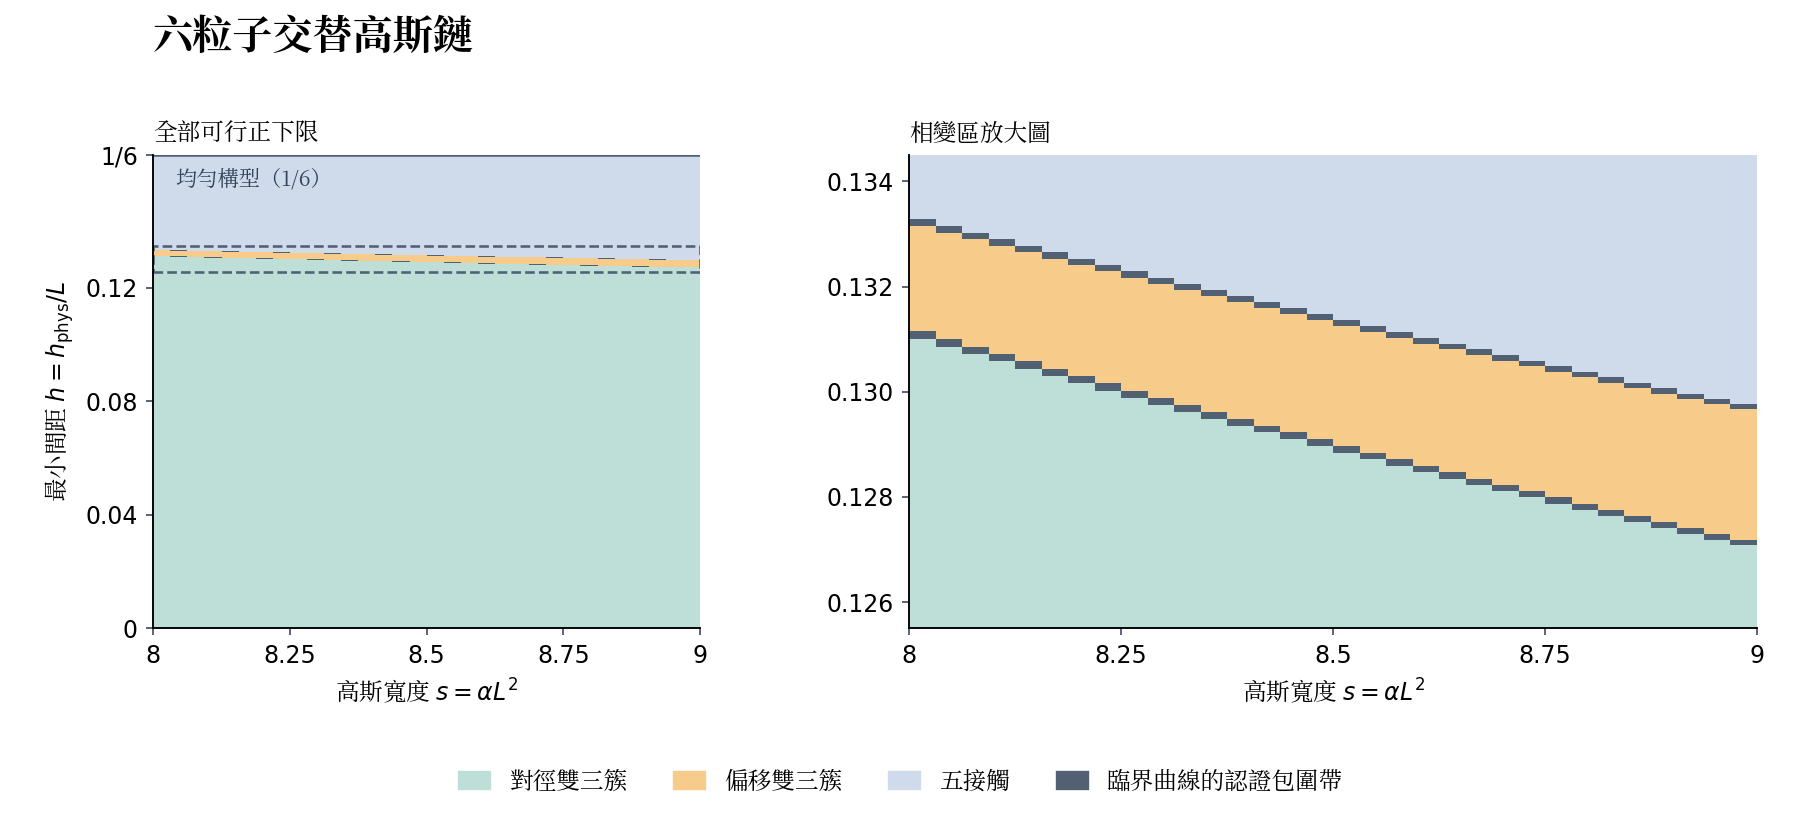
\includegraphics[width=.98\linewidth]{../../research/six-site/width-strip-zh.png}
\else
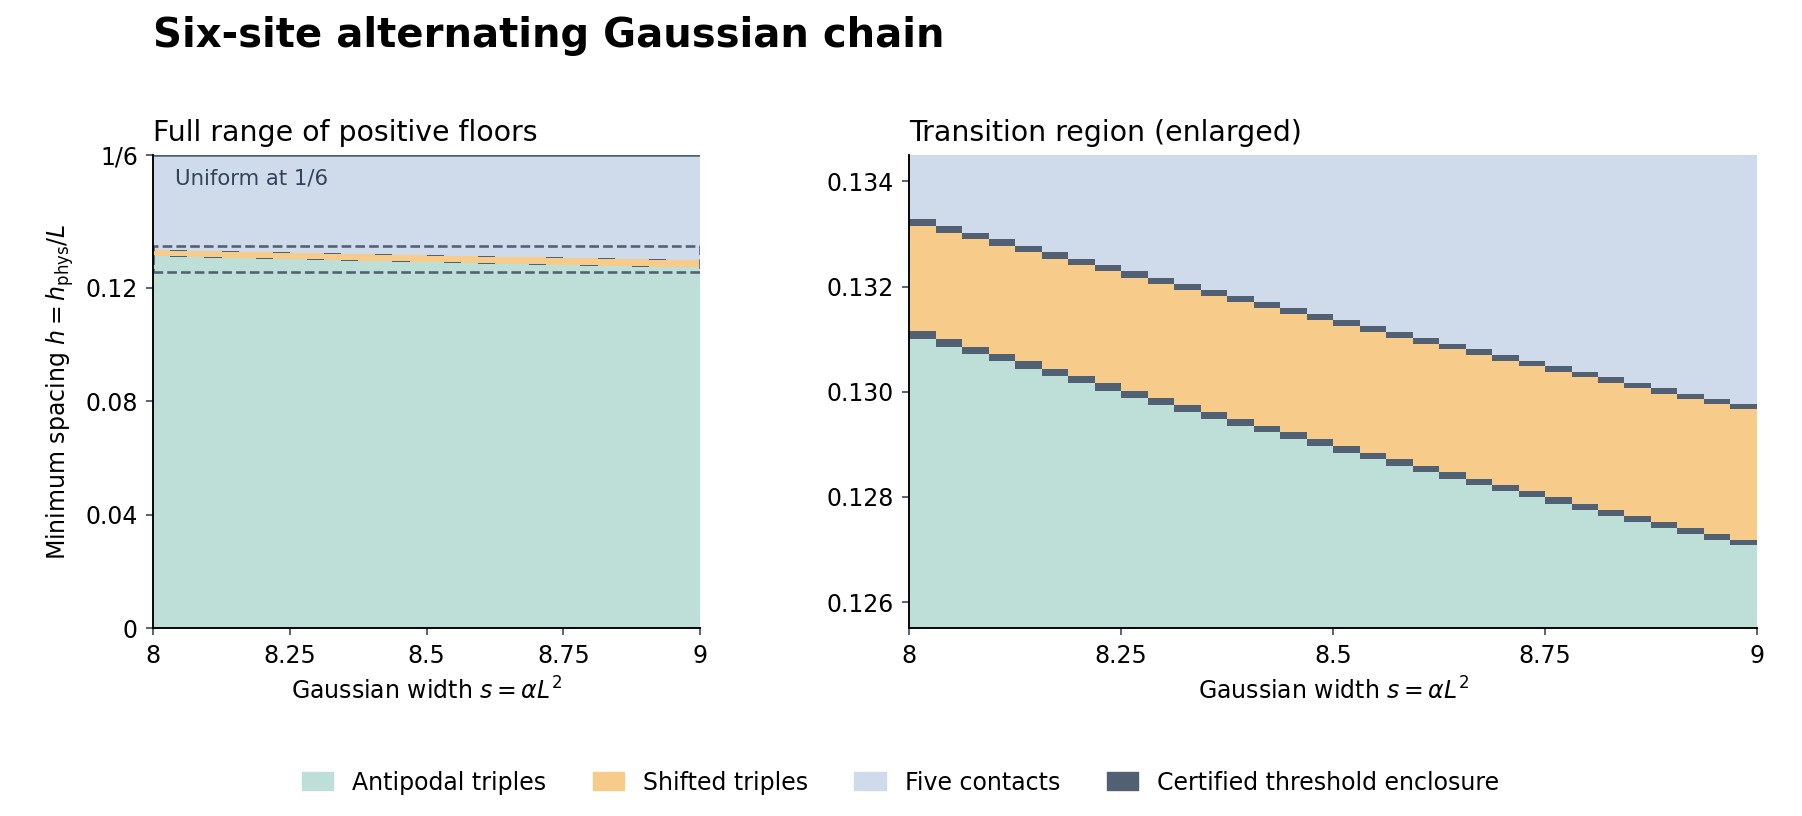
\includegraphics[width=.98\linewidth]{../../research/six-site/width-strip.png}
\fi
\caption{\bi{Global minimizers on $[8,9]$ and an enlargement of the transition region. Green denotes centered, orange shifted, and blue five-contact cells. Dark steps enclose the true curves by monotonicity between consecutive certified endpoints at spacing $1/32$. At $h=1/6$ the cell is uniform.}{寬度 $[8,9]$ 上的全域極小者與相變區放大圖。綠、橙、藍分別為對徑、偏移及五接觸相。相距 $1/32$ 的認證端點及單調性給出深色階梯包圍帶。$h=1/6$ 時構型均勻。}}\label{fig:strip}
\end{figure}


\section{\bi{A different global minimizer at a single width and floor}{單一寬度與下限處的另一種全域極小者}}
\begin{thm}\label{th:point}
\bi{At $N=6$, $s=22$, $h=1/1000$, every minimizing gap word is a cyclic shift of $(h,h,R-h,1/2-R,1/2-R,R-h)$. A representative cell and strict enclosures are}{當 $N=6$、$s=22$、$h=1/1000$，每個極小間隙字均為 $(h,h,R-h,1/2-R,1/2-R,R-h)$ 的循環移位。一組代表與嚴格包圍為}
\begin{align}
 X_*&=(-h,0,h,R,\tfrac12,1-R)\pmod 1,\label{eq:point}\\
 0.249999032167246504146498709394&<R<0.249999032167246504146498709395,\notag\\
 0.66503584451339086827047430&<M_6(1/1000;22)<0.66503584451339086827047431 .\notag
\end{align}
\bi{There is one geometry and two species-preserving orbits, distinguished by the net charge of the triple, even if reflection is allowed.}{幾何形狀唯一；保留電荷種類時，由緊三簇的淨電荷區分為兩個軌道，即使容許反射亦然。}
\end{thm}
\begin{proof}
\bi{\emph{Comparison with the packed face.} Set $G=G_{22}$. Moving the third coordinate of the collision trial in \cite[Eq.~(17)]{infimum} from $125/1000$ to $126/1000$ gives the admissible cell $X=(0,125,126,250,500,750)/1000$. The signed weight of a pair of packed triples with directed center separation $d$ is $2A_n^2(1-\cos(2\pi nd))$. Contracting each triple to its net charge sets $A_n=1$ and gives auxiliary energy $E_0(d)=1+[G(d)-G(0)]/3$. The first nine terms of $E(Y)-E_0$ are nonnegative since $|A_n|\le1$. From $q<3/4$, $c<1$, $A_n^2-1\le8$, the loss in the tail is bounded by $(32/3)(3/4)^{100}/[1-(3/4)^{21}]$. Write $r=\operatorname{dist}(d,\mathbb Z)$. For $r\le1/4$ the nearest image alone exceeds $2e^{-11/2}$; otherwise convexity of $e^{-22u^2}$ on $[1/4,3/4]$ gives the same lower bound from the nearest two. Also $G(0)\le1+2e^{-22}/(1-e^{-66})$. Rational evaluation gives $E(Y)>.669391180769582$ for every $Y$ on the face and $E(X)<.667106810407357$. Thus $X$ beats the whole face by more than $.002284370362225$. The admissible $Z=(0,1,2,251,501,751)/1000$ already has $E(X)-E(Z)>.00207096588405$.}{\emph{能量上界與整族比較。} 記 $G=G_{22}$。將文獻 \cite[式 (17)]{infimum} 碰撞試探的第三個坐標由 $125/1000$ 移至 $126/1000$，得可行構型 $X=(0,125,126,250,500,750)/1000$。兩緊三簇的中點有向間距為 $d$ 時，帶號模態權重為 $2A_n^2(1-\cos(2\pi nd))$。將各簇收縮至淨電荷相當於置 $A_n=1$，輔助能量為 $E_0(d)=1+[G(d)-G(0)]/3$。$E(Y)-E_0$ 的前九項因 $|A_n|\le1$ 皆非負。由 $q<3/4$、$c<1$、$A_n^2-1\le8$，其餘尾項的損失不逾 $(32/3)(3/4)^{100}/[1-(3/4)^{21}]$。設 $r=\operatorname{dist}(d,\mathbb Z)$。若 $r\le1/4$，單一最近像已超過 $2e^{-11/2}$；否則由 $e^{-22u^2}$ 在 $[1/4,3/4]$ 的凸性，最近二像給出同一下界。又 $G(0)\le1+2e^{-22}/(1-e^{-66})$。有理估計得整面 $E(Y)>.669391180769582$、$E(X)<.667106810407357$。故 $X$ 比整個面的任一構型低逾 $.002284370362225$。可行點 $Z=(0,1,2,251,501,751)/1000$ 已有 $E(X)-E(Z)>.00207096588405$。}

\bi{\emph{Global localization.} Cutting at all slack gaps gives one of the twelve cyclic block types in Table~\ref{tab:point}. These exhaust the nonempty subsets of six cuts modulo rotation and reversal, since $6h<1$. For two disjoint contacting pairs, remove them and let $r=1/2-\delta$ be the short distance of the residual opposite pair. The fixed-gauge auxiliary energy is $E_0(r)$. With $K=44$, $\|G''\|_\infty=-G''(0)<K$ by positive Fourier coefficients and the positive noncentral image contributions to $G''(0)$. The two pair self terms and their mixed double difference add at most $4Kh^2$ to the ordered score. On either residual arc of length $u$, the interaction of a removed pair with the residual pair is a first difference of $G(v)-G(u-v)$; its derivative is $G'(v)+G'(u-v)$. The kernel is decreasing up to $1/2$. At most one argument exceeds $1/2$, by at most $\delta$; $G'(1/2)=0$ bounds this derivative by $K\delta$. Adding two pairs in both directions costs at most $4Kh\delta$. The certified signs $G''<0$ on $[0,.1]$, $G'<0$ on $[.1,.25]$, $G''>1$ on $[.25,.5]$ establish monotonicity. They and $G(.25)-G(.5)>1/8$ give $G(r)-G(.5)\ge\delta^2/2$ by two integrations or monotonicity. Completing the square gives}{\emph{全域定位。} 在所有鬆弛間隙切開圓周，得到表~\ref{tab:point} 的十二種循環塊型；因 $6h<1$，它們窮盡六個切口的非空子集在旋轉及反序下的代表。若有兩對不共享粒子的接觸，移去它們後，餘下的異號粒子短弧距離設為 $r=1/2-\delta$，其輔助能量為 $E_0(r)$。取 $K=44$，由 Fourier 係數為正及 $G''(0)$ 非中央像的正貢獻知 $\|G''\|_\infty=-G''(0)<K$。兩對的自身項及其二重差分對有向得分共增加至多 $4Kh^2$。在長 $u$ 的餘下弧上，被移去一對與兩餘點的交互項是 $G(v)-G(u-v)$ 的一階差分，其導數為 $G'(v)+G'(u-v)$。核至 $1/2$ 遞減；兩自變量至多一個超過 $1/2$，且超出至多 $\delta$，由 $G'(1/2)=0$ 得導數至多 $K\delta$。兩對及雙向計數合計至多 $4Kh\delta$。經認證的 $G''<0$ 於 $[0,.1]$、$G'<0$ 於 $[.1,.25]$、$G''>1$ 於 $[.25,.5]$ 給出單調性。以兩次積分或單調性配合 $G(.25)-G(.5)>1/8$ 得 $G(r)-G(.5)\ge\delta^2/2$。完成平方即得}
\[
 E\ge E_0(1/2)+\delta^2/6-2Kh\delta/3-2Kh^2/3
 \ge E_0(1/2)-(2K^2+2K)h^2/3>.66807 .
\]
\bi{If all six gaps are slack, a single-site variation of the ordered score requires $\sigma_i V''(x_i)\le G''(0)$, $V(u)=\sum_j\sigma_j G(u-x_j)$. Truncate $V''$ at degree two to a trigonometric polynomial $T$. Its tail divided by $2c(2\pi)^2$ is at most $54(.64)^9/[1-(4/3)^2(.64)^7]<.63+4(.63)^4$, while $-G''(0)/[2c(2\pi)^2]\ge q+4q^4$, $.63<q<.64$. Thus $\sigma_i T(x_i)<0$ for all six sites. Alternation forces six distinct zeros; multiplication by $e^{4\pi i u}$ gives a nonzero polynomial of degree at most four in $e^{2\pi i u}$. This is impossible.}{若六隙全鬆弛，由有向得分的單粒子變分有 $\sigma_i V''(x_i)\le G''(0)$，其中 $V(u)=\sum_j\sigma_j G(u-x_j)$。截取 $V''$ 至二階三角多項式 $T$。尾項除以 $2c(2\pi)^2$ 後至多為 $54(.64)^9/[1-(4/3)^2(.64)^7]<.63+4(.63)^4$；而 $-G''(0)/[2c(2\pi)^2]\ge q+4q^4$、$.63<q<.64$。所以全部六點皆有 $\sigma_iT(x_i)<0$。符號交替迫使六個相異零點；但乘 $e^{4\pi iu}$ 後得到關於 $e^{2\pi iu}$ 的非零至多四次多項式，矛盾。}
\par
\begin{table}[tbp]\centering
\caption{\bi{Exhaustion at $(22,1/1000)$. Digits count sites in maximal packed blocks.}{參數點 $(22,1/1000)$ 的窮盡分類。每個數字是一個極大緊塊的粒子數。}}\label{tab:point}
\begin{tabular}{lp{.52\linewidth}}\toprule
\bi{Cyclic words}{循環塊長字} & \bi{Certificate}{排除或定位證書}\\\midrule
$6,33,42,51,222,321,411,2121,2211$ & $E>.66807>E(X)$\\
$111111$ & \bi{six zeros of a degree-two trigonometric polynomial}{二次三角多項式須有六個零點}\\
$21111$ & \bi{1,269 boxes, no survivors}{1,269 盒，全部排除}\\
$3111$ & \bi{541 boxes, 10 leaves in the uniqueness region}{541 盒，10 個葉盒進入唯一性區}\\\bottomrule
\end{tabular}\end{table}
\par
\bi{For the last two faces, the block-kernel inequalities of Appendix~\ref{sec:cert} exclude a box if $W<W(X)$ or a two-sided translation violates necessary gradient or curvature conditions. In the single-contact tree the three exclusion counts are $36,283,316$; in the adjacent-contact tree they are $24,158,79$, and the remaining ten closed boxes have all four slack gaps in $[.21,.29]$. No boundary is lost because any newly contacting gap has its own actual block word. A second full cover in block-start coordinates visits 5,638 boxes with $344,32,934,1509$ leaves discarded by order, score, gradient and curvature, and six localized leaves, all of type $3111$. Both covers use $X$ as the feasible bound.}{最後兩面採附錄~\ref{sec:cert} 的塊核估計，若 $W<W(X)$ 或雙向平移違反梯度或曲率必要條件即排除整盒。單接觸樹的三類排除葉數為 $36,283,316$；相鄰雙接觸樹為 $24,158,79$，另十個閉盒內四個鬆弛間隙皆屬 $[.21,.29]$。任何新接觸的邊界點另歸其實際塊長字。另以塊首坐標全域覆蓋 5,638 盒，次序、得分、梯度、曲率分別排除 $344,32,934,1509$ 個葉盒，六個保留葉盒均為 $3111$。兩種覆蓋都以 $X$ 作可行界。}

\bi{\emph{Local shape and equality.} With a $+,-,+$ triple write its coordinates $(-v,u-v,u)$, fixing its signed first moment. The other sites $r,z,t$ have signs $\tau=(-,+,-)$. For short gaps $h\le u,v\le.02$ and the four long gaps in $[.21,.29]$, differentiation of the score gives}{\emph{局部形狀與等號。} 將 $+,-,+$ 三點寫為 $(-v,u-v,u)$，固定其帶號一階矩。其餘點 $r,z,t$ 帶號 $\tau=(-,+,-)$。當短隙 $h\le u,v\le.02$ 且四個長隙在 $[.21,.29]$，對得分微分有}
\[
 W_u/v=\int_0^1\left[G''(u+\lambda v)+
             \sum_{y=r,z,t}\tau_yG''(y-u+\lambda v)\right]\dd\lambda .
\]
\bi{For $W_v/u$ replace the arguments by $v+\lambda u$ and $y+v-\lambda u$. Verified bounds on the three argument ranges are $G''<-38$ on $[0,.04]$, $G''>14$ on $[.21,.33]$, $G''<7$ on $[.42,.58]$. Both derivatives divided by the other gap are $<-59$. Contraction to $u=v=h$ shrinks the external argument intervals and is feasible. Set $C(d)=G(d-h)-G(d)+G(d+h)$. The variable score becomes}{對 $W_v/u$ 將兩個自變量換成 $v+\lambda u$ 與 $y+v-\lambda u$。三段核界為 $G''<-38$ 於 $[0,.04]$、$G''>14$ 於 $[.21,.33]$、$G''<7$ 於 $[.42,.58]$。兩偏導數各除以另一短隙均 $<-59$。收縮至 $u=v=h$ 會縮小外點自變量區間，並保持可行。令 $C(d)=G(d-h)-G(d)+G(d+h)$，可變得分為}
\[
 -C(r)+C(z)-C(t)-G(z-r)+G(t-r)-G(t-z).
\]
\bi{In the convex set where the four consecutive distances of $0,r,z,t$ are in $[.21,.31]$, $C''>14$ on the side distances and $C''<7$ on the diagonals, with the same bounds for $G''$. In the Hessian the four side coefficients are strictly below $-14$, the two diagonal coefficients below 7. Each squared diagonal velocity difference is bounded by the sum of all four squared side differences, averaging the two two-edge paths and applying $(a+b)^2\le2(a^2+b^2)$. Any nonzero velocity after fixing translation has a nonzero side difference. Strict concavity follows. Reflection sends $(r,z,t)$ to $(1-t,1-z,1-r)$, so at a point on its fixed line the differential equals the differential on the averaged, tangent direction. On that line stationarity reads}{在 $0,r,z,t$ 的四個相鄰距離屬於 $[.21,.31]$ 的凸域上，邊距有 $C''>14$，對角距有 $C''<7$，$G''$ 滿足相同界。Hessian 中四邊係數嚴格小於 $-14$，兩對角係數小於 7。對於一條對角，沿兩條二邊路徑分別用 $(a+b)^2\le2(a^2+b^2)$ 再取平均，其速度差平方至多為四邊速度差平方之和。固定平移後任一非零速度至少使一邊有非零速度差，遂得嚴格凹性。反射將 $(r,z,t)$ 送至 $(1-t,1-z,1-r)$，因此在不動直線上一階微分等於其對平均後切向的微分。直線上的駐點條件為}
\begin{equation}\label{eq:force}
 C'(R)-G'(1/2-R)-G'(2R)=0 .
\end{equation}
\bi{The image-sum enclosures give strictly negative and positive signs at the left and right endpoints in \eqref{eq:point}. The root in the convex domain is a full stationary point and strict concavity makes it unique. Compactness supplies a global maximizer and the exhaustive localization puts it in this domain. Substitution of the entire root interval into the fifteen pair terms proves the energy enclosure. In particular $E(X)-M_6>.00207096589396576$. Reflection preserves the charge of the uniquely identifiable triple, whereas global reversal interchanges its two assignments.}{像和包圍在式 \eqref{eq:point} 的左右端點分別給出嚴格負、正號。凸域內的根是完整駐點，且由嚴格凹性唯一。緊性保證全域極大者存在，而窮盡定位迫使它落入此域。將根的整個包圍區間代入十五項配對能量得所述嚴格能量界，特別有 $E(X)-M_6>.00207096589396576$。反射保留唯一可辨緊三簇的淨電荷，整體換號則互換兩種指派。}
\end{proof}


\section{\bi{Counterexamples, conclusions and remaining boundary}{反例、結論及尚待確定的邊界}}
\bi{The hard floor selects exact contacts by a first-order variation; on the six-site strip the remaining freedom is a single relative displacement. A comparison of the two endpoints misses the entire intermediate phase. At $s=8$, $h=263/2000$ and $t=1/1000$, direct rational image sums give $E(Y(h,b))-E(Y(h,0))>23/100000$ and $E(Y(h,0))-E(Y(h,t))>10^{-8}$. At $h=3/20$ the order of the endpoints reverses: the five-contact trial beats the center by more than $.00129689$. At $s=8.5,h=.13$ set $g_i=h+(1-6h)u_i$. The off-face trial $2^{20}u=(0,0,184621,0,1,863954)$ beats the center by more than $.0000876382$, yet loses by more than $6.3349\,10^{-8}$ to the on-face trial $2^{40}u=(905905483609,0,0,193606144167,0,0)$. Each comparison is between explicit cells. The global conclusions require Theorem~\ref{th:strip}.}{硬下限藉一階變分選出精確接觸；在六粒子條帶上，餘下的自由度是一個相對位移。僅比較兩端構型會漏掉整個偏移相。在 $s=8$、$h=263/2000$、$t=1/1000$，有理像和給出 $E(Y(h,b))-E(Y(h,0))>23/100000$ 與 $E(Y(h,0))-E(Y(h,t))>10^{-8}$。在 $h=3/20$ 兩端的次序反轉，五接觸比居中者低逾 $.00129689$。在 $s=8.5,h=.13$，記 $g_i=h+(1-6h)u_i$，面外試探 $2^{20}u=(0,0,184621,0,1,863954)$ 比居中者低逾 $.0000876382$，卻比面內的 $2^{40}u=(905905483609,0,0,193606144167,0,0)$ 高逾 $6.3349\,10^{-8}$。此處是指定構型間的比較；全域結論使用定理~\ref{th:strip}。}

\bi{The collision competitor in \cite{infimum} beats the limiting dipole at width 22. At the positive floor $h=1/1000$, let $K$ be the feasible gap simplex and $F$ the closed packed-triple face with its cyclic copies. Define}{文獻 \cite{infimum} 的碰撞構型在寬度 22 勝過極限偶極。固定正下限 $h=1/1000$，令 $K$ 為可行間隙單純形，$F$ 為緊雙三簇閉面及其循環移位之聯集。定義}
\[
 D(s)=\min_{x\in F}E_s(x)-\min_{x\in K}E_s(x),\qquad
 s_*=\inf\{s>9:D(s)>0\}.
\]
\bi{Joint continuity of the energy and compactness of both fixed sets give continuity of $D$. Theorem~\ref{th:strip} gives $D(9)=0$, and the strict whole-face comparison in Theorem~\ref{th:point} gives $D(22)>0$. The set of widths with strict defeat is open. Its lower boundary $s_*$ remains unknown, as does coexistence there with an off-face minimizer. This definition allows more than one component. Theorem~\ref{th:point} classifies the contact type at the stated pair; an explicit surrounding phase region remains to be determined. For general $N$, Theorem~\ref{th:lock} gives a sufficient small-floor bound and leaves the endpoint of exact locking open.}{能量聯合連續，兩個固定集合皆緊，故 $D$ 連續。定理~\ref{th:strip} 給出 $D(9)=0$，定理~\ref{th:point} 的整面嚴格比較給出 $D(22)>0$。緊面嚴格落敗的寬度構成開集。其下邊界 $s_*$ 的數值，以及該處是否有面外極小者共存，仍待確定。此定義允許多個連通分支。定理~\ref{th:point} 在所述參數點確定接觸類型，周圍相區的顯式範圍仍待求出。對一般 $N$，定理~\ref{th:lock} 給出充分的小間距界，精確鎖定的終點仍未確定。}

\paragraph{\bi{Research and writing disclosure.}{研究及撰寫披露。}}
\bi{AI-assisted work produced trial configurations, symbolic derivations, proof drafts, interval programs and explanatory text at successive stages. This edition used Codex to integrate and translate those local materials, audit the mathematics, compile the articles and coordinate a separate agent review. Trial searches used floating-point arithmetic. Claims of strict inequality rely on analytic estimates or outward interval bounds. The appendix identifies the small formalized portion. The independent review in the archive is an AI review; journal and independent human refereeing remain separate steps.}{各研究階段使用 AI 輔助提出試探構型、推導公式、擬寫證明、編寫區間程序及說明文字。本版以 Codex 整合及翻譯本機底稿、複核數學、編譯論文，並安排獨立 Agent 審閱。試探搜索採浮點算術；嚴格不等式均以解析估計或向外捨入的區間界為依據。附錄逐項說明已形式化的部分。附件所載獨立審查由 AI 完成，期刊與獨立人類同行審查仍待進行。}

\appendix
\section{\bi{Certified bounds on the continuous configuration space}{連續構型空間的嚴格區間證書}}\label{sec:cert}
\bi{\emph{What a terminal box proves.} For $h<1/6$ write $S=1-6h$ and $g_i=h+Su_i$ with $u_i\ge0$, $\sum_i u_i=1$. Put a largest $u_i$ at position 5. The other positive indices form $A\subseteq\{0,\ldots,4\}$. Reflection has eight fixed subsets among 32, hence 20 representatives. The target closed edge and vertex have $A=\{2\}$ and $\varnothing$; 18 supports remain. For $C_k=\{(i,j):i\le k<j\}$, $C_5=\varnothing$, define $d_{ij}=(j-i)h+S\sum_{p=i}^{j-1}u_p$, $w_{ij}=(-1)^{i+j}$. The unordered score with kernel $F_s$ below must satisfy}{\emph{終止盒所證明的命題。} 對 $h<1/6$ 令 $S=1-6h$，$g_i=h+Su_i$、$u_i\ge0$、$\sum_i u_i=1$。將一個最大 $u_i$ 重標在第 5 號間隙，其餘正坐標構成 $A\subseteq\{0,\ldots,4\}$。32 個子集在反射下有 8 個不動者，故有 20 種代表。目標閉邊及頂點對應 $A=\{2\}$ 與空集，尚餘 18 種支撐。對 $C_k=\{(i,j):i\le k<j\}$、$C_5=\varnothing$，記 $d_{ij}=(j-i)h+S\sum_{p=i}^{j-1}u_p$、$w_{ij}=(-1)^{i+j}$。以下文 $F_s$ 作核，無序得分須滿足}
\begin{equation}\label{eq:cuts}
 \sum_{C_k} w_{ij} F_s'(d_{ij})=0,\qquad
 \sum_{C_k\triangle C_l}w_{ij}F_s''(d_{ij})\le0 ,
\end{equation}
\bi{for transfers involving slack gaps (5 to $k$ for the gradient, $k$ to $l$ for curvature). Dividing out $S$ or $S^2$ is legitimate in this range. Both signs of the transfer are feasible in the original simplex even if two largest gaps tie. The cuts alter only crossing pairs; the squared transfer velocity selects the symmetric difference in the curvature. Closed coordinate boxes contain the entire relative-open face. A boundary point where a gap ceases to be slack is tested on its own support. Coordinate sums are intersected with bounds from their complements and the total-sum constraint. A box terminates if empty, strictly beaten by a feasible trial, or violating either necessary condition. Otherwise bisect the longest free coordinate with both children sharing the midpoint. An unresolved box at the minimum step fails the verifier. Success gives a finite proof by induction on the actual trees.}{其中涉及轉移的間隙須鬆弛（一階由第 5 隙轉至 $k$；二階在 $k,l$ 之間）。此時可除以 $S$ 或 $S^2$。即使最長間隙並列，原單純形中仍可雙向變分。只有跨越切口的配對改變，速度平方給出二階式的對稱差。閉坐標盒覆蓋整個面的相對內部；若某鬆隙在邊界變為接觸，該點另由自己的實際支撐處理。坐標和的包圍與補集及總和約束的包圍取交集。空盒、被可行試探嚴格擊敗或違反一項必要條件均可終止，否則沿最長自由坐標對分，兩子盒均含中點。達最小步長仍未判定即驗證失敗。成功時對所生成的有限樹歸納即得覆蓋證明。}

\bi{\emph{Uniform kernel bounds.} On $[\ell,r]$ with midpoint $a$, replace $G_s$ by $F_s=c_a+(c_a q_a)/(c_s q_s)(G_s-c_s)$, $q_s=e^{-\pi^2/s}$, $c_s=\sqrt{\pi/s}$. The slope is positive and the constant in the score is shape-independent. The first harmonic is fixed. Let $D_n$ be the larger absolute difference of $q_s^{n^2-1}$ at either endpoint from its value at $a$. For $j=0,1,2$ use}{\emph{寬度一致的核界。} 在以 $a$ 為中點的 $[\ell,r]$，以 $F_s=c_a+(c_a q_a)/(c_s q_s)(G_s-c_s)$ 代替 $G_s$，其中 $q_s=e^{-\pi^2/s}$、$c_s=\sqrt{\pi/s}$。斜率為正，得分的常數變化與構型無關，第一諧波保持固定。令 $D_n$ 為兩端 $q_s^{n^2-1}$ 與中點值所差的較大絕對值。對 $j=0,1,2$ 用}
\[
 \|F_s^{(j)}-G_a^{(j)}\|_\infty\le
 2c_a q_a\left(\sum_{n=2}^4(2\pi n)^jD_n+
 \frac{(10\pi)^j q_r^{24}}{1-(6/5)^j q_r^{11}}\right).
\]
\bi{The bounds below are in units of $10^{-9}$. On the narrow band they follow instead by differentiating $q_s^{n^2-1}$ and summing the geometric tail relative to width 8. At the reference width tabulate images $|p|\le3$ at mesh $1/8192$. Neighboring Gaussian values are generated by products of ratios whose own ratio is constant. Enclose the starting exponentials by alternating Taylor sums and round each product outwards to units of $10^{-32}$. The derivative multipliers are $1,-2a d,(2ad)^2-2a$ at image argument $d$. Omitted images with $|p|\ge4$ on $[8,9]$ contribute at most $4(324\cdot25+18)2^{-72}<10^{-9}$ in each of the three orders. Spatial extensions use bounds $4,20,150$ on the first three absolute derivatives; at the reference width 8 the original fixed-width table has its own certified bounds. At a score midpoint the code uses the value and slope at the nearest node, a distance at most $1/(2M)$ away, $M=8192$. The first-order Taylor remainder is at most $\|G_a''\|_\infty/(8M^2)$. The node value and slope each have error at most $2\cdot10^{-9}$; flooring the product costs at most one more unit of $10^{-9}$. Widen both the box score and the trial score by $15\epsilon_0$ at the reference center, then bound variation by the widened derivatives. Trial allocations put $u_2=0,1/8,1/4,3/8,1/2$ with the remainder in $u_5$. Only a strict comparison prunes.}{下列各界均以 $10^{-9}$ 為單位。窄帶的界以寬度 8 為基準，對 $q_s^{n^2-1}$ 微分並累加幾何尾項而得。在參考寬度上以 $1/8192$ 網距製作 $|p|\le3$ 的像和表，相鄰高斯值依比值遞推，而比值自身成等比。起始指數用交替 Taylor 級數包圍，每次乘積向外捨入至 $10^{-32}$。對像位差 $d$，導數乘子依次為 $1,-2a d,(2ad)^2-2a$。在 $[8,9]$，被略去的 $|p|\ge4$ 像於三種階數各至多貢獻 $4(324\cdot25+18)2^{-72}<10^{-9}$。空間擴寬採前三階絕對導數界 $4,20,150$；參考寬度 8 的原始核表另有固定寬度認證界。在得分中點用最近節點的函數值及斜率作一階 Taylor 近似。取 $M=8192$，距離至多 $1/(2M)$，故餘項不逾 $\|G_a''\|_\infty/(8M^2)$。節點值及斜率的誤差各至多 $2\cdot10^{-9}$，乘積向下取整再預留一個 $10^{-9}$ 單位。參考中心的盒得分上界及試探下界各擴寬 $15\epsilon_0$，再用擴寬後的導數控制變化。試探取 $u_2=0,1/8,1/4,3/8,1/2$，餘量全在 $u_5$。僅嚴格比較可剪枝。}
\[
\begin{array}{r|rrr}
 [\ell,r]&10^9\epsilon_0&10^9\epsilon_1&10^9\epsilon_2\\\hline
 {[7.99,8.01]}&42761&539098&6806367\\
 {[8,8.5]}&1156027&14580271&184224460\\
 {[8.5,9]}&1309984&16545550&209498225
\end{array}
\]
\par
\begin{table}[tbp]\centering
\caption{\bi{Complete support trees. The last three columns count excluded leaves.}{完整支撐搜尋樹。後三欄為各類排除葉數。}}\label{tab:trees}
\begin{tabular}{lrrrrr}\toprule
$s$ & \bi{floor bands}{下限段} & \bi{boxes}{訪問盒} & \bi{score}{得分} & \bi{gradient}{梯度} & \bi{curvature}{曲率}\\\midrule
$[7.99,8.01]$ &14&6068&261&377&2522\\
$[8,8.5]$ &49&40740&3094&2938&14779\\
$[8.5,9]$ &49&39056&2844&2885&14240\\\bottomrule
\end{tabular}\end{table}
\par
\bi{The 14 narrow bands run from $.10$ to $.12$ in $.002$ steps, then to $.134,.14,.15,1/6$. For the broad bands $300000h$ runs from $21000$ to $49800$ in steps of $600$, then to $50000$. The leaf identity for the two broad trees is $2(5938+5823+29019)-2\cdot49\cdot18=79796$. Independent fixed-width full-simplex verifiers cover $h\ge1/50$ at 8 and $h\ge1/20$ at 9 up to the uniform endpoint. At 9 there are 60,182 visited boxes.}{窄帶的 14 段由 $.10$ 至 $.12$ 以 $.002$ 遞增，再至 $.134,.14,.15,1/6$。廣帶取 $300000h$ 自 $21000$ 至 $49800$ 每次增 $600$，末端再至 $50000$。兩棵廣帶樹的葉數恆等式為 $2(5938+5823+29019)-2\cdot49\cdot18=79796$。獨立固定寬度的全單純形證書於 8 覆蓋 $h\ge1/50$、於 9 覆蓋 $h\ge1/20$ 至均勻端點。寬度 9 的搜尋共訪問 60,182 盒。}

\bi{\emph{A separate rounding proof at width 8.} Round cumulative excesses $M\sum_{k<i}u_k$ down after one common uniform shift in $[0,1)$. All contacts are preserved. For each pair the physical error has mean zero, magnitude below $\rho=S/M$ and variance at most $\rho^2/4$ because a rounded pair difference exceeds its unshifted integer part by a Bernoulli variable whose success probability is the fractional part of the unrounded excess difference. Taylor's theorem for the fifteen unordered terms bounds the expected energy error by $(5/8)\|G''\|_\infty\rho^2$. Consequently some rounded cell has $E_{\rm round}\le E_s(x)+(5/8)\|G''\|_\infty\rho^2$. Finite rational comparisons over $[.08,.10]$ and $[.10,.132]$ confine a minimizer to within $\rho$ in each pair displacement of a viable packed-face grid cell. Transferring length across $m$ sites changes only $m(6-m)$ pair terms; the error in its energy derivative is at most $m(6-m)\|G''\|_\infty\rho/3$. The certified positive release derivatives force all four internal contacts. This second route illustrates why grid energy comparisons alone do not establish a continuum statement.}{\emph{寬度 8 的獨立取整證明。} 對累積餘量 $M\sum_{k<i}u_k$ 加同一個 $[0,1)$ 均勻隨機位移再向下取整，所有接觸均保留。取整後的累積餘量之差等於原差的整數部加上一個 Bernoulli 變量，其成功概率等於原差的小數部。因此各對物理位差誤差期望為零，絕對值小於 $\rho=S/M$，變異數至多 $\rho^2/4$。對十五項無序配對使用 Taylor 定理，期望能量誤差至多 $(5/8)\|G''\|_\infty\rho^2$，故至少一個取整構型滿足單側界 $E_{\rm round}\le E_s(x)+(5/8)\|G''\|_\infty\rho^2$。有理枚舉覆蓋 $[.08,.10]$ 及 $[.10,.132]$，將任一極小者逐對位差定位在某個未被排除的緊面格點的 $\rho$ 內。跨 $m$ 個粒子的轉移只改變 $m(6-m)$ 項，能量導數誤差至多 $m(6-m)\|G''\|_\infty\rho/3$。認證後放寬導數仍為正，迫使四個內間隙精確接觸。此獨立證明亦顯示，由格點能量比較推到連續構型還需要哪些條件。}

\bi{\emph{At width 22.} For blocks of lengths $a,b$ and initial signs $\epsilon_i,\epsilon_j$, form the combined kernel
\[K_{ab}(d)=\sum_{v=0}^{a-1}\sum_{w=0}^{b-1}(-1)^{v+w}G(d+(w-v)h).\] The test for a velocity vector $p$ of whole blocks sums $\epsilon_i\epsilon_j(p_j-p_i)K_{ab}'$ and $\epsilon_i\epsilon_j(p_j-p_i)^2K_{ab}''$ over block pairs. Add the fixed intrablock terms for energy tests. The first cover works in slack gaps of prescribed sum with adjacent-gap reflection symmetry; it checks nonempty proper subsets of blocks moving together. Its node spacing is $1/16000$, derivative intervals in units $10^{-9}$. The second enumerates all cyclic words, propagates $y_{j+1}\ge y_j+a_j h$ for block starts, includes both arc and complementary arc bounds, and also tests opposite block velocities. It uses mesh $1/32000$ and units $10^{-11}$. Retain seven images at each node, adding the two-sided tail $4(1936\cdot25+44)2^{-198}$ for orders zero through two. Compute the signed block sums before interpolating, enclosing the entire interval by widening node extrema by $\|K_{ab}^{(j+2)}\|_\infty/(8M^2)$. In the second cover this norm is bounded by $ab$ times $44,1500,22000$ for $j=0,1,2$. The two covers differ in coordinates, tables and cut directions. Their common analytic assumptions, including the image tail bound, remain open to inspection.}{\emph{寬度 22。} 對長度 $a,b$、起始符號 $\epsilon_i,\epsilon_j$ 的兩塊，合成塊核
\[K_{ab}(d)=\sum_{v=0}^{a-1}\sum_{w=0}^{b-1}(-1)^{v+w}G(d+(w-v)h).\]對整塊速度 $p$，將 $\epsilon_i\epsilon_j(p_j-p_i)K_{ab}'$ 與 $\epsilon_i\epsilon_j(p_j-p_i)^2K_{ab}''$ 分別對所有塊對求和。能量檢驗另加固定的塊內項。第一套覆蓋以總和固定的鬆隙為坐標，利用相鄰外隙反射對稱，檢驗一個非空真子集內的塊同時移動；其節點距 $1/16000$，導數區間單位為 $10^{-9}$。第二套枚舉全部循環字，在塊首坐標上傳播 $y_{j+1}\ge y_j+a_j h$，同時使用弧與補弧界，且另檢驗兩塊相反速度。網距為 $1/32000$，單位 $10^{-11}$。每個節點保留七個像，對零至二階補上雙向尾項 $4(1936\cdot25+44)2^{-198}$。先合成帶號塊和再插值，以 $\|K_{ab}^{(j+2)}\|_\infty/(8M^2)$ 擴寬節點極值，涵蓋整段實數位差。第二套對 $j=0,1,2$ 分別以 $ab$ 乘 $44,1500,22000$ 控制此導數範數。兩套覆蓋使用不同坐標、核表和變分方向；其共用的解析假設，包括像和尾界，均可獨立查核。}

\section{\bi{Formal coverage and reproduction}{形式化範圍與復算指引}}\label{sec:art}
\bi{The file \texttt{AlternatingMoments.lean} proves four declarations. The first two prove the two identities in \eqref{eq:mom}; the general inequality follows analytically by inserting the floor. The other two give the triple variance, its gap derivatives and their lower bounds. Their axiom lists contain exactly \texttt{propext}, \texttt{Classical.choice}, and \texttt{Quot.sound}. The base project's \texttt{Counterexample.lean} separately verifies the earlier four-site Gaussian counterexample. The global contact and phase theorems use the analytic proofs and, where specified, executable interval bounds.}{檔案 \texttt{AlternatingMoments.lean} 證明下列四項聲明。前兩項證明式 \eqref{eq:mom} 的兩個恆等式；一般不等式由代入間距下限解析推出。後兩項證明三粒子方差、兩個間隙導數及其下界。四項公理清單皆恰為 \texttt{propext}、\texttt{Classical.choice} 及 \texttt{Quot.sound}。基礎專案的 \texttt{Counterexample.lean} 另行完整驗證先前的四粒子高斯反例。全域接觸及相圖定理的依據則為上述解析證明及明列的可執行區間界。}

\begin{center}\small
\begin{tabular}{ll}
\texttt{firstMoment} & \texttt{secondMoment}\\
\texttt{tripleVariance\_eq} & \texttt{triple\_gap\_derivatives}
\end{tabular}
\end{center}

\bi{From the root of the public archive, run}{在公開附件的根目錄執行}
\begin{center}\small\texttt{python reproduce.py all -{}-work-dir ../chain-replay}\end{center}
\bi{The setup stage prepares the saved sources and dependencies in the specified work directory before the original verification programs run. The reproduction guide covers the interval certificates, numerical experiments, phase diagram, Lean proofs and both articles. The evidence index identifies the proof inputs for each theorem and distinguishes them from numerical comparisons. The citations and attribution in this edition refer to the source versions preserved in its local research record.}{設定階段先在指定工作目錄準備固定版本的來源及相依項，再執行原驗證程式。復算指南涵蓋區間證書、數值實驗、相圖、Lean 證明及兩份論文。證據索引逐一定理標明證明所用的輸入，並列出另作比較的數值實驗。本版引文與成果歸屬均以本次本地研究記錄所保存的來源版本為據。}


\begingroup
\small
\begin{thebibliography}{10}
\setlength{\itemsep}{2pt}
\bibitem{bkn} L. Bétermin, H. Knüpfer and F. Nolte. Note on crystallization for alternating particle chains. \emph{J. Stat. Phys.} 181 (2020), 803--815. \href{https://doi.org/10.1007/s10955-020-02603-2}{doi:10.1007/s10955-020-02603-2}. arXiv:1804.05743v3.
\bibitem{base} Codex (OpenAI AI model). \emph{A Gaussian counterexample and a Riesz bound for alternating particle chains}. Repository manuscript, \href{https://github.com/xiujiang4/alternating-particle-chains/tree/a48fe4c2623a29dd45edd227410a07baba400250}{revision a48fe4c}.
\bibitem{dilute} OpenAI Codex (submitted by gamehhh7). \emph{Global crystallization of dilute alternating Gaussian chains}. Repository manuscript, \href{https://github.com/xiujiang4/alternating-particle-chains/tree/48e82ad03f1b5f30d6c051b439622cd0bbaf7def}{revision 48e82ad}.
\bibitem{infimum} GPT-6.2 Astra (submitted by Kemody). \emph{The energy infimum for alternating Gaussian chains and the sharp cost of a minimum spacing}. Repository manuscript, Thms.~1--3, \href{https://github.com/Kemody/alternating-particle-chains/blob/7b9bc3e1b13d398a1bf54ab340c18cd3c8f3c88c/en/gaussian-infimum.md}{revision 7b9bc3e}.
\bibitem{four} flyqwq555. \emph{Alternating Chain Lab}, four-site theorem and multi-site experiments. Issue 5, linked proof, Thm.~5, \href{https://github.com/flyqwq555/alternating-chain-lab/tree/53916b8d45785aebaf0059836a3064e80e34f107}{revision 53916b8}.
\bibitem{circle} X. Cabré, G. Csató and A. Mas. Periodic solutions to integro-differential equations: variational formulation, symmetry, and regularity. \emph{Comm. Partial Differential Equations} 50 (2025), Thm.~4.1. \href{https://doi.org/10.1080/03605302.2024.2441851}{doi:10.1080/03605302.2024.2441851}. arXiv:2404.06462.
\bibitem{riesz} M. Christ and M. Iliopoulou. Inequalities of Riesz--Sobolev type for compact connected Abelian groups. \href{https://arxiv.org/abs/1808.08368}{arXiv:1808.08368}.
\bibitem{bipartite} L. Bétermin, L. Šamaj and I. Travěnec. Equidistant versus bipartite ground states for 1D classical fluids at fixed particle density. \emph{Anal. Math. Phys.} 15 (2025), 88. \href{https://doi.org/10.1007/s13324-025-01076-4}{doi:10.1007/s13324-025-01076-4}. arXiv:2502.16639.
\bibitem{prseven} yuri77521 (submitter). Continuous Gaussian displacements for period four. Upstream PR~7, \href{https://github.com/yuri77521/alternating-particle-chains/blob/b7a8ab94064559b8430b6a56749d6f5a1e97d8ef/lean/GaussianDisplacementEnergy.lean}{fixed Lean source, revision b7a8ab9}, theorem \texttt{displacement\_energy\_lt}.
\end{thebibliography}
\endgroup


\end{document}

